\documentclass[12pt]{report}

\input{../macro}


\usepackage[utf8]{inputenc}
\usepackage[T1]{fontenc} 
\usepackage{xspace}
\usepackage[frenchb]{babel}
\usepackage{times}
\usepackage{graphicx}
\usepackage[top=2in, bottom=1.5in, left=1in, right=1in]{geometry}

\graphicspath{{images/}}
\addtocounter{tocdepth}{3}
\setcounter{secnumdepth}{3}
\bibliographystyle{plain}
\renewcommand\thechapter {\Roman{chapter}}

\renewcommand{\baselinestretch}{1.2}

\hyphenation{con-train-te}
 
\begin{document}

\newcommand\university{Université de Grenoble}
\newcommand\school{École doctorale EEATS}
\newcommand\structure{Laboratoire: Inria Grenoble Rhône-Alpes \\ Entreprise: Aldebaran}
\newcommand\auteur{Jory Lafaye}
\newcommand\encadrant{Dr. Pierre-Brice Wieber, Inria\\Dr. Cyrille Collette, Aldebaran\\Dr. Sebastien Dalibard, Aldebaran}
\newcommand\directeur{Dr. Bernard Brogliato, Inria\\~\\~}
\newcommand\titre{Commande des mouvements et de l'équilibre \\d'un robot humanoïde à roues omnidirectionnelles}

\begin{titlepage}

\newcommand{\HRule}{\rule{\linewidth}{0.5mm}} % Defines a new command for the horizontal lines, change thickness here

\center % Center everything on the page
 
%----------------------------------------------------------------------------------------
%	HEADING SECTIONS
%----------------------------------------------------------------------------------------

\textsc{\LARGE \university}\\[0.5cm] 
\textsc{\Large \school}\\[1.5cm] 
\textsc{\Large Thèse CIFRE}\\ 
\textsc{Présentée par}\\[0.5cm] 
\textsc{\Large \auteur}\\ [1.5cm] 
\textsc{\large \structure}\\[0.5cm] 

%----------------------------------------------------------------------------------------
%	TITLE SECTION
%----------------------------------------------------------------------------------------

\HRule \\[0.4cm]
{ \LARGE \bfseries \titre}\\[0.4cm] % Title of your document
\HRule \\[1.5cm]
 
%----------------------------------------------------------------------------------------
%	AUTHOR SECTION
%----------------------------------------------------------------------------------------

\begin{minipage}{0.4\textwidth}
\begin{flushleft} 
\emph{Directeur:}\\
\directeur
\end{flushleft}
\end{minipage}
~
\begin{minipage}{0.4\textwidth}
\begin{flushright} 
\emph{Encadrants:} \\
\encadrant
\end{flushright}
\end{minipage}\\[4cm]

% If you don't want a supervisor, uncomment the two lines below and remove the section above
%\Large \emph{Author:}\\
%John \textsc{Smith}\\[3cm] % Your name

%----------------------------------------------------------------------------------------
%	DATE SECTION
%----------------------------------------------------------------------------------------

%{\large Le \today}\\[3cm] % Date, change the \today to a set date if you want to be precise

%----------------------------------------------------------------------------------------
%	LOGO SECTION
%----------------------------------------------------------------------------------------

%\includegraphics{Logo}\\[1cm] % Include a department/university logo - this will require the graphicx package
 
%----------------------------------------------------------------------------------------

\vfill % Fill the rest of the page with whitespace

\end{titlepage}

\tableofcontents
\listoffigures

%
\newpage\cite{bib.miasa.2010}
%


\addcontentsline{toc}{chapter}{Résumé}

\section{Présentation de la plateforme expérimentale}
	\subsection{Pepper, un robot humanoïde à roues omnidirectionnelles}
	\subsection{Capteurs et actionneurs}
	\subsection{Propriétés mécaniques}	
\section{État de l'art}
	\subsection{Problématiques associées à Pepper}
	\subsection{Commande et équilibre des robots à roues}
		\subsubsection{Les robots à une et deux roues}
		\subsubsection{Les robots à trois roues et plus}
	\subsection{Commande et équilibre des robots bipèdes}
	\subsection{Synthèse et conclusion}
\section{Organisation du document}
\chapter{Modélisation du système}
\section{Choix du modèle et conséquences}
	\subsection{Objectifs}
		L'objectif de ce chapitre est de présenter une modélisation dynamique d'un robot humanoïde possédant une base mobile à roues omnidirectionnelles. 
		Ce modèle doit apporter un bon compromis entre fidélité vis à vis du comportement du robot réel et complexité, qui impacte de manière directe le temps de calcul.
		Notamment, on montre qu'il n'est pas nécessaire de modéliser tout les paramètres du robot : représenter uniquement les dynamiques principales suffit à obtenir un contrôle précis du robot. 
		La section \ref{section.closedloop} détaillera les méthodes de compensation des éléments non modélisés.
	
		\fig{
			\centering
			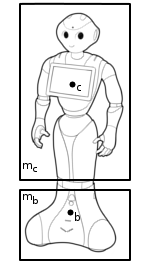
\includegraphics[width=2in]{modele.png}
			\caption{Représentation globale du modèle dynamique.}
			\label{fig.modele}
		}
		
	\subsection{Avantages du modèle}
		
		Le choix se porte sur une modélisation dynamique d'un robot rigide multi-corps. 
		Le modèle présenté \rfi{fig.modele} comporte deux corps. Le premier est attaché à la base mobile, de masse $m_b$ et de position du centre de masse (CoM) $\bar{b}$.
		Le second modélise l'ensemble du reste du robot, de masse $m_c$ et de CoM $\bar{c}$.
		
		Le choix d'un modèle à deux corps permet de prendre en compte la rotation générale du corps du robot autour de la base mobile.
		Cette modélisation est pertinente dans le cas où les bras du robot ne génèrent que peu ou pas de moment angulaire.
		Dans le cas contraire, nous considérerons que les effets parasites dû aux mouvements des bras pourront être compensés correctement par le schéma de contrôle en boucle fermée présenté en section \ref{section.closedloop}.
		Le choix de ce modèle est également conditionné par la répartition massique de la plate-forme expérimentale :
		Elle est principalement concentré en deux zones, qui correspondent aux corps choisis : la base mobile et le torse du robot.	
	
	\subsection{Inconvénients du modèle}
		
		Le choix d'un modèle rigide multi-corps implique que les éléments suivants ne seront pas modélisés :
		\liste{
			\item 	Les différentes élasticités. Les technologies d'actionnement utilisées sur la plate-forme expérimentale ne comportent pas d'élasticités notables.
				Le seul élément compliant est un ensemble de deux bandes élastiques attachées à l'articulation du roulis de la hanche permettant au robot de maintenir une posture droite en l'absence de contrôle du moteur.
				Cet élément est négligeable en terme de dynamique car la raideur associée est très faible.
			\item	Les jeux mécaniques présents sur le robot. Ceux-ci sont présents sur la plate-forme expérimentale, du fait de systèmes de réductions présents entre les moteurs et les articulations basés sur un système d'engrenages.
				Les effets dynamiques parasites apportés par le jeu mécanique ne sont pas négligeables.
				Cependant, il peuvent être compensés de manière suffisamment efficace (plus de détails en section \ref{section.closedloop}) pour que cela soit transparent du point de vue de la commande présentée dans le chapitre \ref{chapitre.commande}.
			\item	Les glissements pouvant survenir entre les roues du robot et le sols ne sont pas modélisés. 
				Ceux-ci peuvent être néanmoins handicapant, car le système devient en partie non-observable en présence de glissement (plus de détails en section \ref{section.observateurbase}).
				Une solution a été apportée en section \ref{section.objectifs3roues} afin de limiter leurs possibilités d'apparition ainsi que leurs impacts sur la dynamique du robot.
			\item	Le nombre de corps choisi pour cette modélisation dynamique est nécessairement plus faible que le nombre de corps réels présents sur le robot, pour des raisons de complexité du modèle.
				Ainsi, tout les effets dynamiques ne pourront pas être représentés. Le choix du nombre de corps, et de leurs propriétés doit permettre de rendre négligeable les dynamiques non modélisées.
				Le développement d'une solution optimale du choix du nombre de corps et de leurs propriété est présenté en annexe \ref{annexe.choixmodele}.
		}
		

	\section{Modélisation dynamique}

		\subsection{Problème de complémentarité mixte}
		
			\subsubsection{Géométrie du robot}
			
		
				On considère le robot modélisé par deux masses-point $\bar{b}$ et $\bar{c}$ de masse associée $m_b$ et $m_c$. 
				Ces corps sont en contact avec le sol par l'intermédiaire de trois points $p_f$, $p_r$ et $p_l$ correspondant aux trois points de contact des roues avec le sol \rfi{fig.bascule}.
				La roue avant gauche correspond au point $p_r$, la roue avant droite au point $p_l$ et la roue arrière au point $p_f$.
				On considère que le système peut être dans quatre mode dynamique différents :
				\liste{
					\item Le robot ne bascule pas et les trois roues sont en contact avec le sol.
					\item Le robot est en rotation vers l'avant autour de l'axe défini par les deux roues avant. On note l'angle de rotation $\psi_f$. La roue arrière est dans ce cas en l'air.
					\item Le robot est en rotation vers la gauche autour de l'axe défini par la roue avant gauche et la roue arrière. On note l'angle de rotation $\psi_l$. La roue avant droite est dans ce cas en l'air.
					\item Le robot est en rotation vers la droite autour de l'axe défini par la roue avant droite et la roue arrière. On note l'angle de rotation $\psi_r$. La roue avant gauche est dans ce cas en l'air.
				}
				Enfin, on la répartition de la masse de chaque corps est concentrée en un seul point. Ainsi, il n'y a aucune inertie de rotation associée à $\bar{b}$ ou $\bar{c}$
		
				\fig{
					\centering
					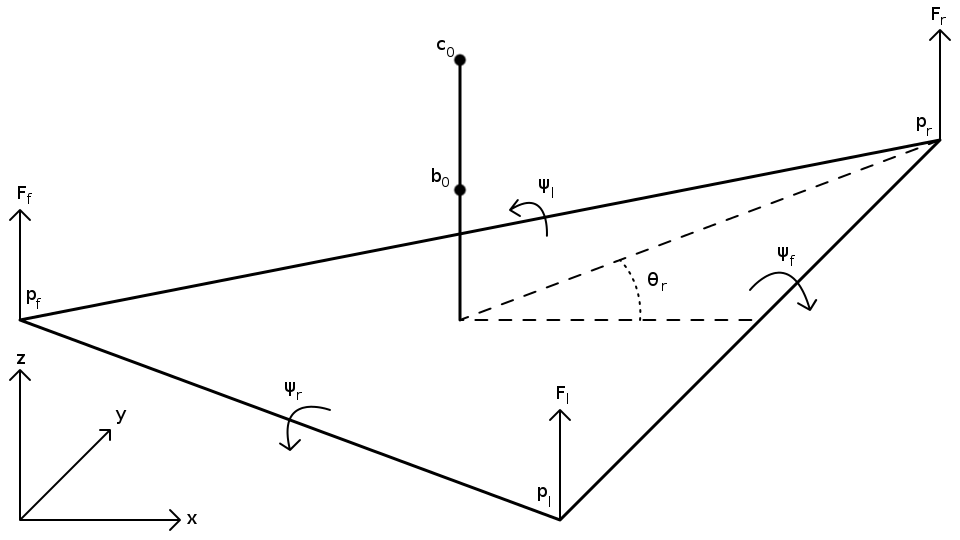
\includegraphics[width=6.5in]{bascule.png}
					\caption{représentation dans le repère $\rep_w$ des points de contacts avec le sol et des angles de basculement.}
					\label{fig.bascule}
				}
			\subsubsection{Cinématique directe}
			
				\subsubsubsection{Notations}
				
				
					Dans la suite, nous considèrerons un repère galiléen fixe orthonormé direct $\rep_w(O, \vec{x},\vec{y},\vec{z})$, $\vec{x}$ étant orienté vers l'avant du robot, $\vec{y}$ vers la gauche, et $\vec{z}$ vers le haut. 
					Ce repère est attaché au sol, $\vec{x}$ et $\vec{y}$ inclus dans le plan, et $\vec{z}$ orthogonal au sol. 
					Celui-ci n'est pas forcément horizontal, ce qui implique que le vecteur gravité ne soit pas forcément orienté selon l'axe $\vec{z}$.
					
					Premièrement, on considère que la position des corps $\bar{c}$ et $\bar{b}$ correspond à la composition de trois éléments \rfi{fig.lagrange}:
					\liste{
						\item $c_0$ et $b_0$ correspondent à la position d'origine de chaque corps par rapport à l'origine. Il est à noter que $c_0^{xy}=b_0^{xy}$.
						\item $\delta_c$ correspond à longueur apportée par l'actionnement des moteurs du robot. On peut noter du fait qu'il n'y a pas d'actionnement possible pour la base mobile, $\delta_b=0$.
						\item $\psi_f$, $\psi_r$ et $\psi_l$ correspondent aux rotations apportées par le basculement du robot sur chaqu'un de ses cotés.
					}
					
					Afin de pouvoir écrire les équations cinématiques, nous avons besoin de définir différentes grandeurs dépendantes de la géométrie du robot \rfi{fig.lagrange}\rfi{fig.bascule}. 
					
					\fig{
						\centering
						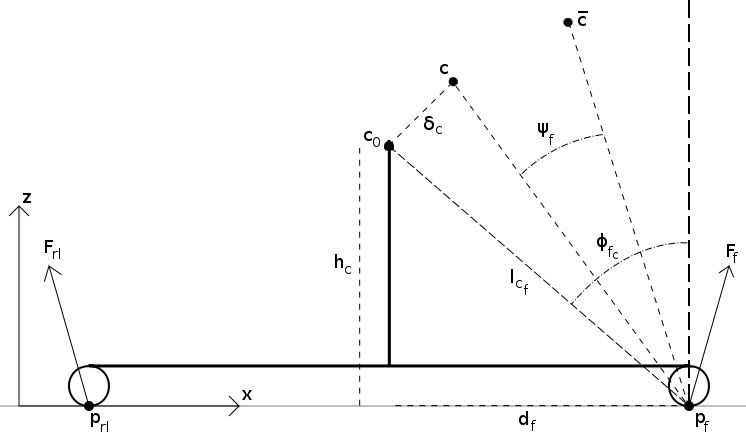
\includegraphics[width=6.5in]{lagrange.png}
						\caption{Projection dans le plan $(O,\vec{x}, \vec{z})$ du modèle du robot. 
							 Représentation des variables relatives au corps $\bar{c}$ et à l'angle $\psi_f$. 
							 Celles relatives à $\bar{b}$, $\psi_r$ et $\psi_l$ ne sont pas représentées, mais correspondent au même schéma.}
						\label{fig.lagrange}
					}
					$\forall i\in\{f,r,l\}$ :
					\liste{
						\item On note $\theta_i$ l'angle que fait le vecteur $\overrightarrow{b_0^{xy}~p_i^{xy}}$ avec l'axe $\vec{x}$. 
						On note $\vec{n_i}$ l'axe résultant et l'axe orthogonal $\vec{t_i}=\vec{z} \times \vec{n_i}$.
						$c_0$ et $b_0$ étant verticalement alignés, il en est de même pour le corps $\bar{c}$.
						On note $\rep_i$ le repère $(O, \vec{n}_i, \vec{t}_i, \vec{z})$.
						\item On note $\phi_{i_b}$ et $\phi_{i_c}$ les angles que font respectivement les vecteurs $\overrightarrow{b_0^{t_iz}~p_i^{t_iz}}$ et $\overrightarrow{c_0^{t_iz}~p_i^{t_iz}}$ avec l'axe $\vec{z}$.
						\item $l_{b_i}$ et $l_{c_i}$ correspondent aux normes des vecteurs $\overrightarrow{b_0^{xyz}~p_i^{xyz}}$ et $\overrightarrow{c_0^{xyz}~p_i^{xyz}}$.
						\item $d_i$ correspond à la norme du vecteur $\overrightarrow{b_0^{xy}~p_i^{xy}}$, qui est la même concernant le corps $\bar{c}$.
						\item $h_b$ et $h_c$ correspondent à la composante selon l'axe $\vec{z}$ des vecteurs $\overrightarrow{b_0^{xyz}~p_i^{xyz}}$ et $\overrightarrow{c_0^{xyz}~p_i^{xyz}}$.
					}
					
					
					Enfin, on note $b$ et $c$ les positions commandées des corps par rapport à l'origine $O$ :
					\eqa{
						b^{xyz} &= b_0^{xyz}\\
						c^{xy} &= c_0^{xy}+\delta_c^{xy}  = b_0^{xy} + \delta_c^{xy} \\
						c^z &= c_0^z + \delta_c^z = b_0^z + h_c + \delta_c^z
					}
					
				\subsubsubsection{Equations cinématiques}
					
					Nous pouvons à présent écrire les équations cinématiques des corps $\bar{c}$ et $\bar{b}$ :
					\eqa{
					\label{eq.cin_cx}
						\bar{c}^x &= c^x + \somme{i\in\{f, r, l\}}{}{d_i\cos(\theta_i) + l_{c_i}\sin(\phi_{i_c}+\psi_i)\cos(\theta_i)}  \\
					\label{eq.cin_cy}
						\bar{c}^y &= c^y + \somme{i\in\{f, r, l\}}{}{d_i\sin(\theta_i) + l_{c_i}\sin(\phi_{i_c}+\psi_i)\sin(\theta_i)} \\
					\label{eq.cin_cz}
						\bar{c}^z &= c^z + \somme{i\in\{f, r, l\}}{}{-h_c + l_{c_i}\cos(\phi_{i_c}+\psi_i)}
					}
					\eqa{
					\label{eq.cin_bx}
						\bar{b}^x &= b^x + \somme{i\in\{f, r, l\}}{}{d_i\cos(\theta_i) + l_{b_i}\sin(\phi_{i_b}+\psi_i)\cos(\theta_i)}  \\
					\label{eq.cin_by}
						\bar{b}^y &= b^y + \somme{i\in\{f, r, l\}}{}{d_i\sin(\theta_i) + l_{b_i}\sin(\phi_{i_b}+\psi_i)\sin(\theta_i)} \\
					\label{eq.cin_bz}
						\bar{b}^z &= b^z + \somme{i\in\{f, r, l\}}{}{-h_b + l_{b_i}\cos(\phi_{i_b}+\psi_i)}
					}
					
					Nous aurons besoin également des équations cinématiques des points $p_{frl}$. $\forall i\in\{f,r,l\}$ :
					
					\eqa{
					\label{eq.cin_px}
						p_{i}^{x} &= b^{x} + d_{i}\cos(\theta_{i}) + l_{b_{i}}\sin(\phi_{i_b}+\psi_{i})\cos(\theta_{i}) \\
					\label{eq.cin_pz}
						p_{i}^{x} &= b^{y} + d_{i}\sin(\theta_{i}) + l_{b_{i}}\sin(\phi_{i_b}+\psi_{i})\sin(\theta_{i}) \\
					\label{eq.cin_py}
						p_{i}^{z} &= b^{z} - h_b + l_{b_{i}}\cos(\phi_{i_b}+\psi_{i})
					}
				
				\subsubsubsection{Hypothèse d'angles de basculements faibles}
				
					Dans la suite, afin de simplifier les formulations des équations de la dynamique, nous allons établir dès maintenant une hypothèse : Les angles $\psi_{frb}$ sont considérés proches de $0$.
					Dans le cas où le robot ne bascule pas, cela est exact. Dans le cas où le robot bascule, on suppose le fait que l'angle de basculement reste faible.
					Nous pouvons donc réécrire les équations cinématiques \rf{eq.cin_cx}\rf{eq.cin_cy}\rf{eq.cin_cz}\rf{eq.cin_bx}\rf{eq.cin_by}\rf{eq.cin_bz} et \rf{eq.cin_px}\rf{eq.cin_py}\rf{eq.cin_pz} en utilisant une approximation du premier ordre :
					\eqa{
					\label{eq.cin_cx_appr}
						\bar{c}^x &= c^x + h_c\somme{i\in\{f, r, l\}}{}{\cos(\theta_i)\psi_i} \\
					\label{eq.cin_cy_appr}
						\bar{c}^y &= c^y + h_c\somme{i\in\{f, r, l\}}{}{\sin(\theta_i)\psi_i} \\
					\label{eq.cin_cz_appr}
						\bar{c}^z &= c^z + \somme{i\in\{f, r, l\}}{}{d_i\psi_i} \\
					\label{eq.cin_bx_appr}
						\bar{b}^x &= b^x + h_b\somme{i\in\{f, r, l\}}{}{\cos(\theta_i)\psi_i} \\
					\label{eq.cin_by_appr}
						\bar{b}^y &= b^y + h_b\somme{i\in\{f, r, l\}}{}{\sin(\theta_i)\psi_i} \\
					\label{eq.cin_bz_appr}
						\bar{b}^z &= b^z + \somme{i\in\{f, r, l\}}{}{d_i\psi_i}
					}

					\eqa{
					\label{eq.cin_px_appr}
						p_{frl}^{x} &= b^{x} - d_{frl}\cos(\theta_{frl}) \\
					\label{eq.cin_py_appr}
						p_{frl}^{y} &= b^{y} - d_{frl}\sin(\theta_{frl}) \\
					\label{eq.cin_pz_appr}
						p_{frl}^{z} &= b^{z} - h_b + 2d_{frl}\psi_{frl} 
					}
			
			\subsubsection{Énergies cinétiques et potentielles}
			
				\subsubsubsection{Contraintes sur le basculement du robot}
				\label{section.contrainte_basculement}
				
					Afin d'exprimer les équations du mouvement du robot, nous allons utiliser la méthode Lagrangienne.
					Celle-ci est pertinente dans notre cas car elle est particulièrement adaptée à la formulation sans ambiguïtés de systèmes dynamiques soumis à des forces de contraintes, comme les forces de réactions dues au sol sur les roues. 
					Pour cela, il nous faut dans un premier temps écrire les équations des énergies cinétiques $T$ et potentielles $V$ du système :
					
					\eqa{
						T &= \frac{1}{2}m_b(\dot{\bar{b}}^{x^2} + \dot{\bar{b}}^{y^2} + \dot{\bar{b}}^{z^2}) + \frac{1}{2}m_c(\dot{\bar{c}}^{x^2} + \dot{\bar{c}}^{y^2} + \dot{\bar{c}}^{z^2}) \\
						V &= m_bg^x\bar{b}^x + m_cg^x\bar{c}^x + m_bg^y\bar{b}^y + m_cg^y\bar{c}^y + m_bg^z\bar{b}^z + m_cg^z\bar{c}^z \\
					}
					avec $g$ le vecteur gravité. On rappelle que le repère $\rep_w$ étant attaché au sol, le vecteur gravité n'est pas forcément orienté selon la direction verticale $\vec{z}$, car le sol peut ne pas être horizontal.
					
					
					Nous allons considérer une autre hypothèse à partir de maintenant : Il ne peut pas y avoir plus d'un seul des angles $\psi_f$, $\psi_r$ et $\psi_l$ non-nul à la fois. 
					Cela correspond à supposer que le robot ne peut basculer que sur deux roues. On ne considère évidement pas le cas où le robot est en chute libre, ainsi que le cas où il ne bascule que sur une seule roue.
					On justifie cela par le fait que sa construction mécanique ne permet pas au robot de basculer sur une roue, sauf s'il subit une perturbation extrêmement forte.
					
					
					On obtient donc la contrainte suivante :
					\eq{
						\label{eq.contrainte_psi_ij}
						\forall (i,j)\in\{f, r, l\},~ i\neq j,~~ \psi_i\psi_j=0
					}
					
				\subsubsubsection{Formulation des énergies cinétiques et potentielles}
				
					En dérivant les équations cinématiques \rf{eq.cin_cx_appr}\rf{eq.cin_cy_appr}\rf{eq.cin_cz_appr}\rf{eq.cin_bx_appr}\rf{eq.cin_by_appr}\rf{eq.cin_bz_appr} et en utilisant la contrainte précédente \rf{eq.contrainte_psi_ij}, nous pouvons exprimer les vitesses des corps $\bar{c}$ et $\bar{b}$ élevés au carré.
					\eqa{
						\dot{\bar{c}}^{x^2} &= \dot{c}^{x^2} + h_c^2\somme{i\in\{f, r, l\}}{}{\cos(\theta_i)^2\dot{\psi}_i^2} + 2h_c\dot{c}^x\somme{i\in\{f, r, l\}}{}{\cos(\theta_i)\dot{\psi}_i} \\
						\dot{\bar{c}}^{y^2} &= \dot{c}^{y^2} + h_c^2\somme{i\in\{f, r, l\}}{}{\sin(\theta_i)^2\dot{\psi}_i^2} + 2h_c\dot{c}^y\somme{i\in\{f, r, l\}}{}{\sin(\theta_i)\dot{\psi}_i}\\
						\dot{\bar{c}}^{z^2} &= \dot{c}^{z^2} + \somme{i\in\{f, r, l\}}{}{d_i^2\dot{\psi}_i^2} + 2\dot{c}^{z}\somme{i\in\{f, r, l\}}{}{d_i\dot{\psi}_i} \\
						\dot{\bar{b}}^{x^2} &= \dot{b}^{x^2} + h_b^2\somme{i\in\{f, r, l\}}{}{\cos(\theta_i)^2\dot{\psi}_i^2} + 2h_b\dot{b}^x\somme{i\in\{f, r, l\}}{}{\cos(\theta_i)\dot{\psi}_i} \\
						\dot{\bar{b}}^{y^2} &= \dot{b}^{y^2} + h_b^2\somme{i\in\{f, r, l\}}{}{\sin(\theta_i)^2\dot{\psi}_i^2} + 2h_b\dot{b}^y\somme{i\in\{f, r, l\}}{}{\sin(\theta_i)\dot{\psi}_i}\\
						\dot{\bar{b}}^{z^2} &= \dot{b}^{z^2} + \somme{i\in\{f, r, l\}}{}{d_i^2\dot{\psi}_i^2} + 2\dot{b}^{z}\somme{i\in\{f, r, l\}}{}{d_i\dot{\psi}_i}
					}
			
				
					Voici donc la formulation des énergies cinétiques et potentielles en fonction des variables du système :
					
					\eqa{
						\nonumber T &= \frac{1}{2}m_b(\dot{b}^{x^2}+\dot{b}^{y^2}+\dot{b}^{z^2}) + \frac{1}{2}m_c(\dot{c}^{x^2}+\dot{c}^{y^2}+\dot{c}^{z^2}) + \frac{1}{2}(m_bh_b^2+m_ch_c^2)\somme{i\in\{f, r, l\}}{}{\dot{\psi}_i^2}\\
						\nonumber  &+ \frac{1}{2}(m_c+m_b)\somme{i\in\{f, r, l\}}{}{d_i^2\dot{\psi}_i^2}  + (m_ch_c\dot{c}^z+m_bh_b\dot{b}^z)\somme{i\in\{f, r, l\}}{}{d_i\dot{\psi}_i} \\
					\label{eq.T}
						&+ (m_bh_b\dot{b}^x+m_ch_c\dot{c}^x)\somme{i\in\{f, r, l\}}{}{\cos(\theta_i)\dot{\psi}_i} + (m_bh_b\dot{b}^y+m_ch_c\dot{c}^y)\somme{i\in\{f, r, l\}}{}{\sin(\theta_i)\dot{\psi}_i} \\
						\nonumber\\
						\nonumber V &= m_bg^xb^x + m_cg^xc^x + m_bg^yb^y + m_cg^yc^y + m_bg^zb^z + m_cg^zc^z \\
						\nonumber &+ (m_bg^x h_b + m_cg^x h_c)\somme{i\in\{f, r, l\}}{}{\cos(\theta_i)\psi_i} + (m_bg^y h_b + m_cg^y h_c)\somme{i\in\{f, r, l\}}{}{\sin(\theta_i)\psi_i} \\
					\label{eq.V}
						&+(m_b+m_c)g^z\somme{i\in\{f, r, l\}}{}{d_i\psi_i}
					}			
					
			
			\subsubsection{Coordonnées généralisées et Lagrangien}
			
				L'étape suivante dans la méthode Lagrangienne est d'exprimer l'équation du Lagrangien en fonction des coordonnées généralisées choisies.
				
				Habituellement, le choix des coordonnées généralisées correspondent aux degrés de libertés du système. 
				Afin de faciliter la formulation du modèle, nous allons plutôt utiliser le jeu de coordonnées $q$ suivant :
				\eq{
					q = \tr{\mat{b^x & b^y & b^z & c^x & c^y & c^z & \psi_f & \psi_r & \psi_l} }
				}
				
				Le choix d'utiliser les trois angles $\psi_{frl}$ pour représenter la rotation du système autour des trois directions possible permettra par la suite d'exprimer plus simplement les équations de la dynamique.
				
				Le Lagrangien $L$ du système est exprimé à partir des énergies cinétiques et potentielles de la façon suivante :
				\eq{
					L = T - V
				}
				
			\subsubsection{Application du principe de moindre action}	
			
				\subsubsubsection{Définitions}
				
					On défini l'action du système comme l'intégrale temporelle du Lagrangien. 
					Le principe de moindre action énonce que, dans le cas d'un système Lagrangien, l'action est stationnaire. Le plus souvent, cela correspond à un minimum, d'où le terme de ``moindre action''.
					
					Résoudre ce système emmène aux équations d'Euler-Lagrange, équivalentes du principe fondamental de la dynamique de Newton. 
					Dans le cas d'un système contraint par des forces de contact, on écrit :
					\eq{
					\label{eq.lagrange}
						\frac{d}{dt}\frac{\partial L}{\partial \dot{q}} + \frac{\partial L}{\partial q} = \somme{i\in\{f,r,l\}}{k\in\{x,y,z\}}{\frac{\partial p_{i}^k}{\partial q}F_{p_{i}}^k}
					}
					
					Afin de clarifier l'écriture des équations de la dynamique, on pose :
					\eqa{
						m_{hc} &= m_ch_c \\
						m_{hb} &= m_bh_b \\
						m_{q} &= m_{hc}h_c+m_{hb}h_b \\
						m_t &= m_c+m_b \\
						C_{\theta_i} &= \cos(\theta_i) \\
						S_{\theta_i} &= \sin(\theta_i)
					}
				
				\subsubsubsection{Équations de la dynamique}
				
					Les éléments de l'équation \rf{eq.lagrange} peuvent être calculés à l'aide des équations des énergies \rf{eq.T}\rf{eq.V} ainsi que des équations cinématiques \rf{eq.cin_px_appr}\rf{eq.cin_py_appr}\rf{eq.cin_pz_appr} :
					\eqa{
						\label{eq.T_lagrange}
						\frac{d}{dt}\frac{\partial L}{\partial \dot{q}} &=
						\mat{
							m_b\ddot{b}^x+m_bh_b\somme{i\in\{f, r, l\}}{}{\cos(\theta_i)\ddot{\psi}_i} \\
							m_b\ddot{b}^y+m_bh_b\somme{i\in\{f, r, l\}}{}{\sin(\theta_i)\ddot{\psi}_i} \\
							m_b\ddot{b}^z+m_bh_b\somme{i\in\{f, r, l\}}{}{d_i\ddot{\psi}_i} \\
							m_c\ddot{c}^x+m_ch_c\somme{i\in\{f, r, l\}}{}{\cos(\theta_i)\ddot{\psi}_i} \\
							m_c\ddot{c}^y+m_ch_c\somme{i\in\{f, r, l\}}{}{\sin(\theta_i)\ddot{\psi}_i} \\
							m_c\ddot{c}^z+m_ch_c\somme{i\in\{f, r, l\}}{}{d_i\ddot{\psi}_i} \\
							(m_q + m_td^2_f)\ddot{\psi}_f + m_{hb}(C_{\theta_f}\ddot{b}^x+S_{\theta_f}\ddot{b}^y-d_f\ddot{b}^z) + m_{hc}(C_{\theta_f}\ddot{c}^x+S_{\theta_f}\ddot{c}^y+d_f\ddot{c}^z) \\
							(m_q + m_td^2_r)\ddot{\psi}_r + m_{hb}(C_{\theta_r}\ddot{b}^x+S_{\theta_r}\ddot{b}^y-d_r\ddot{b}^z) + m_{hc}(C_{\theta_r}\ddot{c}^x+S_{\theta_r}\ddot{c}^y+d_r\ddot{c}^z) \\
							(m_q + m_td^2_l)\ddot{\psi}_l + m_{hb}(C_{\theta_l}\ddot{b}^x+S_{\theta_l}\ddot{b}^y-d_l\ddot{b}^z) + m_{hc}(C_{\theta_l}\ddot{c}^x+S_{\theta_l}\ddot{c}^y+d_l\ddot{c}^z)
						},
						\\
						\label{eq.V_lagrange}
						\frac{\partial L}{\partial q} &= \mat{
							m_bg^x \\
							m_bg^y \\
							m_bg^z \\
							m_cg^x \\
							m_cg^y \\
							m_cg^z \\
							(m_{hc} + m_{hb})\cos(\theta_f)g^x + (m_{hc} + m_{hb})\sin(\theta_f)g^y + m_td_fg^z \\
							(m_{hc} + m_{hb})\cos(\theta_r)g^x + (m_{hc} + m_{hb})\sin(\theta_r)g^y + m_td_rg^z \\
							(m_{hc} + m_{hb})\cos(\theta_l)g^x + (m_{hc} + m_{hb})\sin(\theta_l)g^y + m_td_lg^z
						},
					}
					\eq{
						\label{eq.P_lagrange}
						\frac{\partial p_{frl}^x}{\partial q} = \mat{
							1\\
							0 \\
							0 \\
							0 \\
							0 \\
							0 \\
							0 \\
							0 \\
							0 \\
						},
						\frac{\partial p_{frl}^y}{\partial q} = \mat{
							0\\
							1 \\
							0 \\
							0 \\
							0 \\
							0 \\
							0 \\
							0 \\
							0 \\
						},
						\frac{\partial p_f^z}{\partial q} = \mat{
							0 \\
							0 \\
							1 \\
							0 \\
							0 \\
							0 \\
							2d_f \\
							0 \\
							0 \\
						},
						\frac{\partial p_r^z}{\partial q} = \mat{
							0 \\
							0 \\
							1 \\
							0 \\
							0 \\
							0 \\
							0 \\
							2d_r \\
							0 \\
						},
						\frac{\partial p_l^z}{\partial q} = \mat{
							0 \\
							0 \\
							1 \\
							0 \\
							0 \\
							0 \\
							0 \\
							0 \\
							2d_l \\
						}
					}
					
				\subsubsubsection{Formulation standard}
				
					Les équations de la dynamique \rf{eq.lagrange} peuvent à présent être réécrites en utilisant la formulation standard utilisée en robotique :
					\eq{
					\label{eq.formulation_standard}
						M \ddot{q} - f(q) = \tr{J}(q)\lambda
					}
					où, en identifiant avec les équations \rf{eq.T_lagrange}\rf{eq.V_lagrange}\rf{eq.P_lagrange} :
					\eqa{
						\lambda &= \tr{\mat{F_{p_{l}}^x & F_{p_{r}}^x & F_{p_{b}}^x & F_{p_{l}}^y & F_{p_{r}}^y & F_{p_{b}}^y & F_{p_{l}}^z & F_{p_{l}}^z & F_{p_{b}}^z}}\\
						M&=\mat{
							M_{bc} & M_{c\psi} \\ 
							\tr{M}_{c\psi} & M_\psi
						}, 
						M_{\psi} = \mat{
							m_q+m_td_f^2 & 0 & 0 \\
							0 & m_q+m_td_r^2 & 0 \\
							0 & 0 & m_q+m_td_l^2 
						},
						\\
						M_{bc} &= \mat{
							m_b & 0 & 0 & 0 & 0 & 0 \\
							0 & m_b & 0 & 0 & 0 & 0 \\
							0 & 0 & m_b & 0 & 0 & 0 \\
							0 & 0 & 0 & m_c & 0 & 0 \\
							0 & 0 & 0 & 0 & m_c & 0 \\
							0 & 0 & 0 & 0 & 0 & m_c
						},
						M_{c\psi} = \mat{
							m_{hb}C_{\theta_f} & m_{hb}C_{\theta_r} & m_{hb}C_{\theta_l} \\
							m_{hb}S_{\theta_f} & m_{hb}S_{\theta_r} & m_{hb}S_{\theta_l} \\
							m_{hb}d_f & m_{hb}d_r & m_{hb}d_l \\
							m_{hc}C_{\theta_f} & m_{hc}C_{\theta_r} & m_{hc}C_{\theta_l} \\
							m_{hc}S_{\theta_f} & m_{hc}S_{\theta_r} & m_{hc}S_{\theta_l} \\
							m_{hc}d_f & m_{hc}d_r & m_{hc}d_l
						}, \\
					}
					\eqa{
						f(q) &= \mat{
							m_b g^x \\ 
							m_b g^y \\ 
							m_b g^z \\ 
							m_c g^x \\ 
							m_c g^y \\ 
							m_c g^z \\ 
							(m_{hc} + m_{hb})\cos(\theta_f)g^x + (m_{hc} + m_{hb})\sin(\theta_f)g^y + m_td_fg^z \\
							(m_{hc} + m_{hb})\cos(\theta_r)g^x + (m_{hc} + m_{hb})\sin(\theta_r)g^y + m_td_rg^z \\
							(m_{hc} + m_{hb})\cos(\theta_l)g^x + (m_{hc} + m_{hb})\sin(\theta_l)g^y + m_td_lg^z
						},\\
						\tr{J}(q) &= \mat{
							1 & 1 & 1 & 0 & 0 & 0 & 0 & 0 & 0 \\
							0 & 0 & 0 & 1 & 1 & 1 & 0 & 0 & 0 \\
							0 & 0 & 0 & 0 & 0 & 0 & 1 & 1 & 1 \\
							0 & 0 & 0 & 0 & 0 & 0 & 0 & 0 & 0 \\
							0 & 0 & 0 & 0 & 0 & 0 & 0 & 0 & 0 \\
							0 & 0 & 0 & 0 & 0 & 0 & 0 & 0 & 0 \\
							0 & 0 & 0 & 0 & 0 & 0 & 2d_f & 0 & 0 \\
							0 & 0 & 0 & 0 & 0 & 0 & 0 & 2d_r & 0 \\
							0 & 0 & 0 & 0 & 0 & 0 & 0 & 0 & 2d_l \\
						}
					}
					
			\subsubsection{Contraintes de complémentarité mixte}
			
				Afin de compléter la formulation de la dynamique, il reste maintenant à utiliser les \textit{a priori} que l'on dispose sur notre système et formuler les contraintes de complémentarité mixte.
				
				Dans un premier temps, le robot n'a pas la possibilité de pénétrer dans le sol, nous avons donc :
				\eq{
					\forall i\in\{f,r,l\}, \psi_i \geq 0
				}
				
				Aussi, lorsque que le robot bascule sur un des axes $\psi_{frl}$, la force résultante sur la roue opposée est nulle :
				\eq{
					\forall i\in\{f,r,l\}, (\psi_i > 0) \then F_i^{xyz} = 0
				}
				
				Ensuite, lorsque le robot est en contact avec le sol, les forces verticales sur les points de contacts sont nécessairement positives :
				\eq{
					\forall i\in\{f,r,l\}, F_i^z \geq 0
				}
				
				Enfin, nous avons défini en section \rf{section.contrainte_basculement} que le robot ne peut pas basculer sur plus d'un des trois axes à la fois :
				\eq{
					\forall (i, j) \in \{f,r,l\},~ i\neq j, ~~ \psi_i\psi_j = 0
				}
				
				Nous pouvons donc exprimer les contraintes de complémentarité mixte pour le système :
				\eq{
				\label{eq.contrainte_complementarite}
					\forall (i, j) \in \{f,r,l\},~ i\neq j, 
					\lst{
						0 \le \psi_i \perp \psi_j \ge 0 \\
						0 \le \psi_i \perp F_i^z \ge 0 \\
						\psi_i F_i^x = 0 \\
						\psi_i F_i^y = 0
					}
				}
				
			\subsubsection{Synthèse}
			
				Dans cette section, nous avons dans un premier temps défini les équations cinématiques associées au modèle du robot.
				Cela nous a permit d'établir une formulation Lagrangienne de la dynamique, puis de l'identifier à la formulation standard des systèmes mécaniques en robotique.
				Enfin, les \textit{a priori} que nous connaissons concernant le système dynamique nous ont permit d'établir des contraintes de complémentarité mixte sur celui-ci.
				
				
				
				Sans ces contraintes, il aurait été possible de résoudre analytiquement les équations temporelles du mouvement. Cependant, la présence de celles-ci imposent une résolution particulière.
				Une première approche, qui sera développée dans les sections suivantes, est d'énoncer d'autres \textit{a priori} afin de fixer le problème de complémentarité
				(par exemple, en considérant que le robot n'est pas en possibilité de basculer, ou est en état de basculement sur un axe). 
				
				Ces approches ne permettent cependant pas de résoudre le problème complet. 
				Nous détaillerons dans la section \rf{section.modelisation_unifiee} une méthode de résolution du système complet \rf{eq.formulation_standard}\rf{eq.contrainte_complementarite}.
		
		\subsection{Cas où les trois roues sont en contact avec le sol}
			
			\subsubsection{Modèle dynamique}
				
				Lorsque le robot est en situation nominale, ses trois roues sont en contact avec le sol. 
				Les mouvements contrôlés du robot ne doivent également pas le faire basculer sur deux roues.
				Il est donc pertinent de modéliser le système dynamique dans le cas où les trois roues sont en contact avec le sol, 
				car en l'absence de forte perturbations, le contrôleur développé en section \rf{section.mpc_trois_roues} assure cette hypothèse.
			
				Définir le fait que le robot est en contact avec le sol avec ces trois roues permet de résoudre le problème de complémentarité de la façon suivante :
				\eq{
					\psi_{f} = \psi_{r} = \psi_{l} = 0
				}
				
				Ainsi, le jeu de variables $q$ devient :
				\eq{
					q = \tr{\mat{b^x & b^y & b^z & c^x & c^y & c^z}}
				}
				et l'on peut écrire le modèle dynamique correspondant :
				\eq{
				\label{eq.modele_trois_roues}
					M \ddot{q} - f(q) = \tr{J}(q)\lambda
				}
				avec :			
				\eqa{
					q_i &= \tr{\mat{b^x & b^y & b^z & c^x & c^y & c^z}} \\
					\lambda &= \tr{\mat{F_{p_{l}}^x & F_{p_{r}}^x & F_{p_{b}}^x & F_{p_{l}}^y & F_{p_{r}}^y & F_{p_{b}}^y & F_{p_{l}}^z & F_{p_{l}}^z & F_{p_{b}}^z}}\\
				\label{eq.force_contrainte_trois_roues}
					F_{p_{f}}^z &\ge 0,~~ F_{p_{r}}^z \ge 0,~~ F_{p_{l}}^z \ge 0 \\
					M &= \mat{
						m_b & 0 & 0 & 0 & 0 & 0 \\
						0 & m_b & 0 & 0 & 0 & 0 \\
						0 & 0 & m_b & 0 & 0 & 0 \\
						0 & 0 & 0 & m_c & 0 & 0 \\
						0 & 0 & 0 & 0 & m_c & 0 \\
						0 & 0 & 0 & 0 & 0 & m_c
					},
				}
				\eqa{
					f(q) &= \mat{
						m_b g^x \\ 
						m_b g^y \\ 
						m_b g^z \\ 
						m_c g^x \\ 
						m_c g^y \\ 
						m_c g^z 
					},
					\tr{J}(q) = \mat{
						1 & 1 & 1 & 0 & 0 & 0 & 0 & 0 & 0 \\
						0 & 0 & 0 & 1 & 1 & 1 & 0 & 0 & 0 \\
						0 & 0 & 0 & 0 & 0 & 0 & 1 & 1 & 1 \\
						0 & 0 & 0 & 0 & 0 & 0 & 0 & 0 & 0 \\
						0 & 0 & 0 & 0 & 0 & 0 & 0 & 0 & 0 \\
						0 & 0 & 0 & 0 & 0 & 0 & 0 & 0 & 0 
					}
				}
			
			\subsubsection{Définition du Centre de Pression}
			
				Dans le cas d'un système dont les positions des forces de contact sont définis sur un plan, il est possible de définir une grandeur nommé Centre de Pression $d^{xy}$ (CoP).
				Le CoP correspond au point dans le plan où le moment angulaire de la résultante des forces de contact est nul.
				La propriété essentielle du CoP est que celui est toujours défini à l'intérieur du polygone de l'enveloppe convexe définie par la position des forces de contact.
				Cela est dû aux contraintes de non-pénétration dans le sol des forces de contact \rf{eq.force_contrainte_trois_roues}.
				Lorsque le CoP est strictement à l'intérieur de ce polygone de support, le robot ne peut pas basculer sur deux roues.
				
				Ainsi, l'utilisation du CoP permet de manipuler de façon pertinente la somme des forces de contact afin de permettre au robot de ne jamais basculer de lui-même.
				Son expression est la suivante :
				\eq{
					d^{xy} = \frac{\somme{i\in\{f,r,l\}}{}{(p \times F)^{xy}}}{\somme{i\in\{f,r,l\}}{}{F_i^z}}
				}
				
			
			\subsubsection{Principe du moment angulaire}
			
				Le modèle de notre robot n'est pas un système fermé. Il n'y a donc pas de conservation du moment angulaire intrinsèque : Le lagrangien n'est pas invariant par rotation.
				Cependant, notre système est soumis à deux types de forces différentes : La première est due à la gravité, et dérive donc d'un potentiel, les secondes sont dues à des efforts de contacts, qui sont des contraintes concernant le sstème.
				Il est possible d'exprimer le principe du moment angulaire dans ce cas là, celui-ci se formule alors :
				
				\eq{
					q \times \prt{\dfrac{d}{dt}\dfrac{\partial L}{\partial \dot{q}} - \dfrac{\partial L}{\partial q}}  = \somme{i\in\{f,r,l\}}{}{p_i \times F}
				}
				
				En utilisant l'équation du modèle dynamique \rf{eq.modele_trois_roues}, on peut donc écrire le principe du moment angulaire autour des axes $\vec{y}$ et $\vec{x}$ :
				\eqa{
				\label{eq.moment_y_trois_roues}
					m_b(\ddot{b}^z-g^z)b^x -m_b(\ddot{b}^x-g^x)b^z + m_c(\ddot{c}^z-g^z)c^x - m_c(\ddot{c}^x-g^x)c^z &= \somme{i\in\{f,r,l\}}{}{p_i^xF_i^z-p_i^zF_i^x} \\
				\label{eq.moment_x_trois_roues}
					m_b(\ddot{b}^z-g^z)b^y -m_b(\ddot{b}^y-g^y)b^z + m_c(\ddot{c}^z-g^z)c^y - m_c(\ddot{c}^y-g^y)c^z &= \somme{i\in\{f,r,l\}}{}{p_i^yF_i^z-p_i^zF_i^y}
				}
				
			\subsubsection{Formulation du Centre de Pression et simplifications}
			
				On rappelle les équations du mouvement sur l'axe $\vec{z}$ \rf{eq.modele_trois_roues} :
				\eq{
				\label{eq.dyn_z_trois_roues}
					m_b(\ddot{b}^z-g^z) + m_c(\ddot{c}^z-g^z) = \somme{i\in\{f,r,l\}}{}{F_i^z}
				}
			
				En utilisant les équations résultantes du principe du moment angulaire autour des axes $\vec{y}$ et $\vec{x}$ \rf{eq.moment_y_trois_roues}\rf{eq.moment_x_trois_roues} ainsi que l'équation \rf{eq.dyn_z_trois_roues}, on peut formuler le CoP de la façon suivante :	
				\eq{
				\label{eq.cop_trois_roues}
					d^{xy} = \frac{m_b(\ddot{b}^z-g^z)b^{xy} -m_b(\ddot{b}^{xy}-g^{xy})b^z + m_c(\ddot{c}^z-g^z)c^{xy} - m_c(\ddot{c}^{xy}-g^{xy})c^z}  {m_b(\ddot{b}^z-g^z) + m_c(\ddot{c}^z-g^z)} \\
				}
				
				Notre objectif va être maintenant de linéariser l'équation \rf{eq.cop_trois_roues} par rapport aux variables commandées $c^{xy}$ et $b^{xy}$.
				Cela va nous permettre d'utiliser un contrôleur basé sur un système linéaire, ce qui est généralement beaucoup plus efficace en terme de temps de calcul qu'un contrôleur basé sur un système non-linéaire.
				
				On peut dans un premier temps noter que $b^z$ est constant à la hauteur $h_b$, car $b=b_0$. Ensuite, on contraint $c^z$ à être constant à la hauteur $h_c$.
				Enfin, on considère la gravité orientée selon l'axe $\vec{z}$ : $g=\tr{\mat{0, 0, -g_n}}$, avec $g_n = \norm{g}$, ce qui correspond à un sol horizontal.
				
				En utilisant ces \textit{a priori}, l'équation de la dynamique \rf{eq.cop_trois_roues} se réécrit :
				
				\eq{
					d^{xy} = \frac{m_bgb^{xy} -m_b\ddot{b}^{xy}h_b + m_cgc^{xy} - m_c\ddot{c}^{xy}h_c}  {(m_b + m_c)g} 
				}
				
				Enfin, les trois contraintes \rf{eq.force_contrainte_trois_roues} impliquent que $d^{xy}$ est à l'intérieur du triangle défini par les trois points de contacts :
				\eqa{
					d^{xy} \times (p_r^{xy}-p_f^{xy}) &\ge 0 \\
					d^{xy} \times (p_l^{xy}-p_r^{xy}) &\ge 0 \\
					d^{xy} \times (p_f^{xy}-p_l^{xy}) &\ge 0
				}
			
			\newpage
			~
			\newpage
			

		
		\subsection{Le robot bascule sur deux roues}

			On résout la complémentarité :
			\eq{
				\forall (i,j,k)\in\{f,r,l\}, i\neq j\neq k,~ \psi_{jk} = 0, F_i^{xyz} = 0
			}
			
			Le modèle dynamique devient :
			\eq{
				M \ddot{q} - f(q) = \tr{J}(q)\lambda
			}
			
			En identifiant :
			\eqa{
				q_i &= \tr{\mat{b^x & b^y & b^z & c^x & c^y & c^z & \psi_i}} \\
				\lambda &= \tr{\mat{F_{p_{j}}^x & F_{p_{k}}^x & F_{p_{j}}^y & F_{p_{k}}^y & F_{p_{j}}^z & F_{p_{k}}^z}}\\
				M &= \mat{
					m_b & 0 & 0 & 0 & 0 & 0 & m_{hb}C_{\theta_i} \\
					0 & m_b & 0 & 0 & 0 & 0 & m_{hb}S_{\theta_i} \\
					0 & 0 & m_b & 0 & 0 & 0 & m_{hb}d_i \\
					0 & 0 & 0 & m_c & 0 & 0 & m_{hc}C_{\theta_i} \\
					0 & 0 & 0 & 0 & m_c & 0 & m_{hc}S_{\theta_i} \\
					0 & 0 & 0 & 0 & 0 & m_c & m_{hc}d_i \\
					m_{hb}C_{\theta_i} & m_{hb}S_{\theta_i} & m_{hb}d_i & m_{hc}C_{\theta_i} & m_{hc}S_{\theta_i} & m_{hc}d_i & m_q+m_td_i^2
				},\\
				f(q) &= \mat{
					m_b g^x \\ 
					m_b g^y \\ 
					m_b g^z \\ 
					m_c g^x \\ 
					m_c g^y \\ 
					m_c g^z \\ 
					(m_{hc} + m_{hb})\cos(\theta_i)g^x + (m_{hc} + m_{hb})\sin(\theta_i)g^y + m_td_ig^z \\
				},\\
				\tr{J}(q) &= \mat{
					1 & 1 & 0 & 0 & 0 & 0 \\
					0 & 0 & 1 & 1 & 0 & 0 \\
					0 & 0 & 0 & 0 & 1 & 1 \\
					0 & 0 & 0 & 0 & 0 & 0 \\
					0 & 0 & 0 & 0 & 0 & 0 \\
					0 & 0 & 0 & 0 & 0 & 0 \\
					0 & 0 & 0 & 0 & 2d_j & 0 \\
					0 & 0 & 0 & 0 & 0 & 2d_k \\
				}
			}
			
			Principe du moment angulaire autour de l'axe $y$ et $x$ :
			\eqa{
				 \nonumber&m_b(\ddot{b}^z-g^z)b^x + m_bh_bd_i\ddot\psi_i\prt{b^x+h_b\cos(\theta_i)\psi_i} -m_b(\ddot{b}^x-g^x)b^z - m_bh_b\cos(\theta_i)\ddot\psi_ib^z\\
				 \nonumber+&m_c(\ddot{c}^z-g^z)c^x + m_ch_cd_i\ddot\psi_i\prt{c^x+h_c\cos(\theta_i)\psi_i} - m_c(\ddot{c}^x-g^x)c^z - m_ch_c\cos(\theta_i)\ddot\psi_ic^z\\
				 =& \somme{s\in\{j,k\}}{}{p_s^xF_s^z-p_s^zF_s^x}
			}
			\eqa{
				 \nonumber&m_b(\ddot{b}^z-g^z)b^y + m_bh_bd_i\ddot\psi_i\prt{b^y+h_b\sin(\theta_i)\psi_i} -m_b(\ddot{b}^y-g^y)b^z - m_bh_b\sin(\theta_i)\ddot\psi_ib^z\\
				 \nonumber+&m_c(\ddot{c}^z-g^z)c^y + m_ch_cd_i\ddot\psi_i\prt{c^y+h_b\sin(\theta_i)\psi_i} - m_c(\ddot{c}^y-g^y)c^z - m_ch_c\sin(\theta_i)\ddot\psi_ic^z\\
				 =& \somme{s\in\{j,k\}}{}{p_s^yF_s^z-p_s^zF_s^y}
			}
			
			Equation du mouvement sur l'axe $z$ :
			\eq{
				m_b(\ddot{b}^z-g^z) + m_bh_bd_i\ddot\psi_i + m_c(\ddot{c}^z-g^z) + m_ch_cd_i\ddot\psi_i = \somme{s\in\{j,k\}}{}{F_s^z}
			}
			
			Equation du CoP $d^{xy}$ :
			
			\eq{
				d^{xy} = \frac{\somme{i\in\{f,r,l\}}{}{p^{xy} \times F^{xy}}}{\somme{i\in\{f,r,l\}}{}{F_i^z}}
			}
			
			\eqa{
				\nonumber d^x &= \frac{m_b\prt{\ddot{b}^z-g^z+h_bd_i\ddot\psi_i}\prt{b^x+h_b\cos(\theta_i)\psi_i} - m_b\prt{\ddot{b}^x-g^x + h_b\cos(\theta_i)\ddot\psi_i}b^z}
				           {m_b(\ddot{b}^z-g^z) + m_c(\ddot{c}^z-g^z) + (m_bh_b+m_ch_c)d_i\ddot\psi_i} \\
				    &+ \frac{m_c\prt{\ddot{c}^z-g^z+h_cd_i\ddot\psi_i}\prt{c^x+h_c\cos(\theta_i)\psi_i} - m_c\prt{\ddot{c}^x-g^x + h_c\cos(\theta_i)\ddot\psi_i}c^z}
				           {m_b(\ddot{b}^z-g^z) + m_c(\ddot{c}^z-g^z) + (m_bh_b+m_ch_c)d_i\ddot\psi_i}
			}
			\eqa{
				\nonumber d^y &= \frac{m_b\prt{\ddot{b}^z-g^z+h_bd_i\ddot\psi_i}\prt{b^y+h_b\sin(\theta_i)\psi_i} - m_b\prt{\ddot{b}^y-g^y + h_b\sin(\theta_i)\ddot\psi_i}b^z}
				           {m_b(\ddot{b}^z-g^z) + m_c(\ddot{c}^z-g^z) + (m_bh_b+m_ch_c)d_i\ddot\psi_i} \\
				    &+ \frac{m_c\prt{\ddot{c}^z-g^z+h_cd_i\ddot\psi_i}\prt{c^y+h_b\sin(\theta_i)\psi_i} - m_c\prt{\ddot{c}^y-g^y + h_c\sin(\theta_i)\ddot\psi_i}c^z}
				           {m_b(\ddot{b}^z-g^z) + m_c(\ddot{c}^z-g^z) + (m_bh_b+m_ch_c)d_i\ddot\psi_i}
			}

			Les variables contrôlées sont directement $c^{xy}, b^{xy}$. $b^z$ est constant à la hauteur $h_b$ et on contraint $c^z$ à être constant à la hauteur $h_c$.
			De plus, la gravité est considérée selon l'axe z : $g=\tr{\mat{0, 0, -g}}$. Enfin, on considère $d_i=0$, ce qui correspond à négliger $d_i$ devant $h_b$ et $h_c$.
			
			\eqa{
				\nonumber d^x &= \frac{m_bg\prt{b^x+h_b\cos(\theta_i)\psi_i} + m_cg\prt{c^x+h_c\cos(\theta_i)\psi_i}}{(m_b+m_c)g} \\
				    &- \frac{m_bh_b\prt{\ddot{b}^x + h_b\cos(\theta_i)\ddot\psi_i}- m_ch_c\prt{\ddot{c}^x + h_c\cos(\theta_i)\ddot\psi_i}}{(m_b+m_c)g}
			}
			\eqa{
				\nonumber d^y &= \frac{m_bg\prt{b^y+h_b\sin(\theta_i)\psi_i} + m_cg\prt{c^y+h_c\sin(\theta_i)\psi_i}}{(m_b+m_c)g} \\
				    &- \frac{m_bh_b\prt{\ddot{b}^y + h_b\sin(\theta_i)\ddot\psi_i}- m_ch_c\prt{\ddot{c}^y + h_c\sin(\theta_i)\ddot\psi_i}}{(m_b+m_c)g}
			}
			
			Les deux contraintes $ F^z_{jk} \ge 0$ impliquent que $d^{xy}$ est dans le segment défini par les deux points de contact. 
			Pour assurer le maximum de robustesse, on choisi de contraindre le CoP au centre du segment :
			\eqa{
				d^x &= b^x + d_i\cos(\theta_i) \\
				d^y &= b^y + d_i\sin(\theta_i) 
			}
			
			On peut donc réécrire les équations précédente pour faire apparaitre la dynamique de $\psi_i$ par rapport à celles de $b$ et $c$ :
			\eqa{
				\label{eq.model_psi_x}
				\nonumber &(m_bh_b+m_ch_c)g\cos(\theta_i)\psi_i - (m_bh_b^2+m_ch_c^2)\cos(\theta_i)\ddot\psi_i \\
				=&~m_bh_b\ddot{b}^x + m_ch_c\ddot{c}^x - m_cg(c^x-b^x) - (m_c+m_b)gd_i\cos(\theta_i)
			}
			\eqa{
				\label{eq.model_psi_y}
				\nonumber &(m_bh_b+m_ch_c)g\sin(\theta_i)\psi_i - (m_bh_b^2+m_ch_c^2)\sin(\theta_i)\ddot\psi_i \\
				=&~m_bh_b\ddot{b}^y + m_ch_c\ddot{c}^y - m_cg(c^y-b^y) - (m_c+m_b)gd_i\sin(\theta_i)
			}
			
			Un rotation autour de l'axe $z$ de l'angle $\theta_i$ fait apparaitre, en combinant les équations \rf{eq.model_psi_x} et \rf{eq.model_psi_y} sous la forme \rf{eq.model_psi_n} $=cos(\theta_i)$\rf{eq.model_psi_x}$+\sin(\theta_i)$\rf{eq.model_psi_y} :
			\eq{
				\mat{c^x\\c^y} = \mat{\cos(\theta_i) & -\sin(\theta_i) \\ \sin(\theta_i) & \cos(\theta_i)} \mat{c^n \\c^t} 
			}
			\eq{
				\label{eq.model_psi_n}
				(m_bh_b+m_ch_c)g\psi_i - (m_bh_b^2+m_ch_c^2)\ddot\psi_i = m_bh_b\ddot{b}^n + m_ch_c\ddot{c}^n - m_cg(c^n-b^n) - (m_c+m_b)gd_i
			}
	\section{Modélisation de la dynamique future}
		\subsection{Nécessité de prédire le futur}

			- Les contraintes dynamiques sont trop fortes pour autoriser un contrôle sans prédiction du futur à haute accélération.

			- Démontrer en calculant les accélérations limites dans différents cas

			- Non nécéssité d'un modèle dynamique précis dans le futur (feedback, on ne calcule que la première commande)

			- Permet d'assurer une stabilité à long terme (quelques secondes)
		\subsection{Choix de la dynamique d'extrapolation}

			- Contraintes : Linéarité entre les variables / accélérations continues donc polynome d'ordre 3

			- Formulation de l'équation d'état

			- Calcul des dérivées

		\subsection{Formulation du modèle prédictif}

			- Formulation du modèle prédictif

			- Problème de controlabilité dans le cas de basculement.
			
			- Inversions de matrice
\chapter{Commande par modèle prédictif}
\label{chapitre.commande}
	\section{Principe}
	
		L'objectif de ce chapitre est de présenter la loi de commande permettant de réaliser les mouvements et l'équilibre d'un robot humanoïde à roues omnidirectionnelles.
		Dans le chapitre \rf{chapitre.modele}, nous avons développé un modèle du robot utilisant deux corps.
		Les contraintes de complémentarités dues aux forces de contact nous ont emmené à modéliser le robot en deux parties : lorsque celui-ci possède ses trois roues en contact avec le sol, et lorsqu'il bascule sur deux de ses roues.
		Ensuite de quoi, nous avons montré qu'il est important de modéliser la dynamique dans le futur à cause des contraintes sur le CoP, qui limitent fortement les mouvements réalisables par le robot.
		Enfin, deux équations prédictives de la dynamique ont été formulées :
		\liste{
			\item Dans le cas où le robot possède trois roues sur le sol, l'équation \rf{eq.dyn_cop_pred} exprime la relation entre la position du CoP et la dynamique des corps du robot.
			\item Dans le cas où le robot bascule sur deux roues, l'équation \rf{eq.dyn_tilt_pred} exprime la dynamique de l'angle de basculement en fonction de celle des corps du robot.
		}
		
		Nous avons donc choisi de réaliser une loi de commande optimale basée sur un modèle prédictif linéaire en les variables de commande, soumis à des contraintes linéaires.
		La fonction objectif de cette commande optimale est basée sur la minimisation d'une norme d'ordre $2$, permettant la convergence d'une grandeur d'erreur vers $0$, utilisés notamment dans une tâche de suivi de trajectoire.
		
		L'interêt de l'aspect prédictif de cette commande est de pouvoir utiliser les connaissances que l'on a sur le comportement dynamique du système ainsi que sur les mouvements demandés, pour prévoir et adapter en avance les trajectoires résultantes.
		Cela permet d'obtenir une meilleure réalisation des objectifs dans le temps. 
		Cette adaptation est nécessaire lorsque les contraintes du système réduisent de beaucoup l'ensemble des trajectoires atteignables instantanément par les corps du robot, ce qui est notre cas.
	
	\section{Outil mathématique et contraintes associées}
	
		Notre objectif est d'exécuter la loi de commande en temps réel sur la plate-forme expérimentale. 
		Il est donc important d'utiliser un outil mathématique de calcul qui permette cela.
		Le système étant fortement contraint (Position du CoP, limites articulaires, limites dynamique des moteurs), nous ne pouvons disposer d'une solution analytique.
		Une méthode de résolution numérique du problème doit donc être envisagée.
		
		Nous avons donc choisi d'utiliser la méthode de la programmation quadratique sous contraintes linéaires (QP).
		Cette méthode de formulation d'un problème d'optimisation permet de minimiser une fonction objectif quadratique en les variables d'optimisation, celles-ci étant soumises à des contraintes d'inégalités linéaires :
		\eq{
			\lst{
				\min\limits_x \prt{\tr{x}Qx+\tr{\rho}x} \\
				v^- \leq Vx \leq v^+
			}
		}
		avec $x$ le vecteur des variables d'optimisation, $Q$ la matrice hessienne, $\rho$ le vecteur linéaire, $V$ la matrice des contrainte et $v^+$ et $v^-$ les vecteurs des bornes des contraintes.
		
		Une fois le problème posé, un solveur de QP permet, en temps réel, de calculer la solution du problème de minimisation en un certain nombre d'itérations, dépendant principalement des contraintes.
		L’annexe \rf{annexe.qp} détaille les méthodes de résolutions d'un problème quadratique.


	\section{Formulation des problèmes d'optimisations}
		\subsection{Introduction}
		
 			De par les contraintes de complémentarité mixtes du modèle \rf{eq.contrainte_complementarite}, ainsi que des contraintes cinématiques du robot et de la base mobile, il n'est pas possible de résoudre simplement l'équation de la dynamique.
 			Nous avons donc choisi de présenter la commande du robot sous la forme de trois contrôleurs supervisés par une machine à état.
 			
 			Le premier contrôleur correspond au cas où le robot possède les trois roues sur le sol, en utilisant la dynamique de l'équation \rf{eq.dyn_cop_pred}. 
 			En l'absence de perturbation emmenant le CoP sur le bord du polygone de support, 
 			ce contrôleur seul est suffisant et assure que le robot ne basculera pas lors de ses mouvements.
 			
 			Le problème se corse lorsqu'une perturbation fait basculer le robot.
 			Nous avons donc choisi de définir deux autres contrôleurs permettant de gérer cette situation. 
 			Le second correspond au moment où le robot est en train de basculer, en utilisant la dynamique de l'équation \rf{eq.dyn_tilt_pred}.
 			Le dernier permet d'assurer une transition cohérente entre les deux modèles.
 			
 			Le modèle dynamique de basculement \rf{eq.dyn_tilt_pred} ne prend pas en compte la présence du sol, qui ajoute une force compensant la gravité lorsque l'angle de basculement atteind $0$.
 			Cette absence d'information emmène le second contrôleur à se comporter de manière non désirée à de faibles angles de basculement, en compensant la gravité par l'accélération de la base mobile, au lieu de ``laisser tomber'' le robot sur le sol en laissant les forces de contact la compenser par la suite.
 			Ce troisième contrôleur est là pour gérer ce cas particulier afin d'assurer une bonne transition.

		\subsection{Lorsque les trois roues sont en contact avec le sol}
			\label{section.mpc_trois_roues}
			\subsubsection{Formulation des objectifs}
			\label{section.objectifs3roues}

				Lorsque les trois roues sont en contact avec le sol, nous pouvons définir trois objectifs de commande :
				\liste{
					\item Assurer le suivi d'une trajectoire de référence. Nous avons fait le choix d'un asservissement position/vitesse de la trajectoire de la base mobile.
					\item Assurer une bonne robustesse aux perturbations. Cet objectif consiste à conserver le meilleur potentiel d'action du robot.
					      Ce potentiel d'action est limité par les contraintes sur le CoP $D^{xy}$, ainsi que les contraintes cinématiques entre le corps du robot et la base mobile.
					      En optimisant au plus loin possible le CoP $D^{xy}$ ainsi que le CoM $C^{xy}$ du corps du robot de leurs contraintes respectives, nous assurons une robustesse optimale face à une perturbation inconnue.
					\item Assurer la stabilité numérique de la commande optimale. Cela peut être réalisé en minimisant le carré des variables de commande $X$.
				}
				
				Dans la suite, nous noterons $O_i$ l'objectif $i$. Il correspond à la norme élevée au carré d'une fonction des variables de commande. Il s'écrit de la façon suivante :
				\eq{
					O_i = \frac{1}{2}\norm{f_i(X)}^2
				}
				puis, en utilisant la notation des problèmes quadratiques :
				\eq{
					O_i = \frac{1}{2}\tr{X}Q_iX + \tr{\rho}_iX + \epsilon_i
				}
				avec $Q_i$ une matrice symétrique définie positive (dite Hessienne), $\rho_i$ un vecteur et $\epsilon_i$ un scalaire constant.
				Nous ne détaillerons pas l'expression de $\epsilon_i$ car ce terme n'a pas d'impact pas dans la minimisation des l'objectif $O_i$ (Plus de détails en section \rf{section.qp_3roues}).
				
				On rapelle le vecteur de commande dans le cas où le robot à les trois roues en contact avec le sol :
				\eq{
					X = \tr{\mat{\dddot{C}^x & \dddot{C}^y & \dddot{B}^x & \dddot{B}^y}}
				}
				\subsubsubsection{Suivi de trajectoire}
				
					L'objectif principal de la commande est d'assurer un suivi de trajectoire de la base mobile, par rapport à une trajectoire de référence $(B^{xy}_{ref}, \dot{B}^{xy}_{ref})$ définie sur l'ensemble de l'horizon de prédiction.
					
					Nous pouvons donc écrire les objectifs $O_1$ et $O_2$, qui correspondent respectivement au suivi de trajectoire en position et en vitesse :
					\eqa{
						O_1 &= \frac{1}{2}\norm{B^{xy}-B^{xy}_{ref}}^2 = \frac{1}{2}\tr{X}Q_1X + \tr{\rho}_1X + \epsilon_1 \\
						O_2 &= \frac{1}{2}\norm{\dot{B}^{xy}-\dot{B}^{xy}_{ref}}^2 = \frac{1}{2}\tr{X}Q_2X + \tr{\rho}_2X + \epsilon_2
					}
					avec:
					\eqa{
						Q_1 &= \mat{
							0 & 0 & 0 & 0 \\
							0 & 0 & 0 & 0 \\
							0 & 0 & \tr{U}_b U_b & 0 \\
							0 & 0 & 0 & \tr{U}_b U_b
						},~~
						\rho_1 = \mat{
							0 \\
							0 \\
							\tr{U}_b(S_b\hat{b}^x-B^x_{ref}) \\
							\tr{U}_b(S_b\hat{b}^y-B^y_{ref})
						} \\
						Q_2 &= \mat{
							0 & 0 & 0 & 0 \\
							0 & 0 & 0 & 0 \\
							0 & 0 & \tr{U}_{\dot{b}} U_{\dot{b}} & 0 \\
							0 & 0 & 0 & \tr{U}_{\dot{b}} U_{\dot{b}}
						},~~
						\rho_2 = \mat{
							0 \\
							0 \\
							\tr{U}_{\dot{b}}(S_{\dot{b}}\hat{b}^x-\dot{B}^x_{ref}) \\
							\tr{U}_{\dot{b}}(S_{\dot{b}}\hat{b}^y-\dot{B}^y_{ref})
						}
					}
				
				\subsubsubsection{Robustesse aux perturbations}
				
					L'objectif suivant de la commande est d'assurer une bonne robustesse face à une perturbation inconnue.
					Dans ce cas, la meilleure robustesse est atteinte lorsque le CoP $D^{xy}$ et le CoM du corps du robot $C^{xy}$ est au plus loin des contraintes, donc au centre de la base mobile aux points $B^{xy}$.
					
					Nous pouvons donc définir deux objectifs $O_3$ et $O_4$, qui correspondent respectivement au centrage du CoP et à celui du CoM du corps du robot :
					\eqa{
						O_3 &= \frac{1}{2}\norm{D^{xy}-B^{xy}}^2 = \frac{1}{2}\tr{X}Q_3X + \tr{\rho}_3X + \epsilon_3 \\
						O_4 &= \frac{1}{2}\norm{C^{xy}-B^{xy}}^2 = \frac{1}{2}\tr{X}Q_4X + \tr{\rho}_4X + \epsilon_4
					}
					avec:
					\eqa{
					\nonumber
						Q_3 &= \mat{
							\tr{U}_{dc}U_{dc} & 0 & \tr{U}_{dc}(U_{db}-U_b) & 0 \\
							0 & \tr{U}_{dc}U_{dc} & 0 & \tr{U}_{dc}(U_{db}-U_b) \\
							(\tr{U}_{db}-U_b)U_{dc} & 0 & (\tr{U}_{db}-\tr{U}_b)(U_{db}-U_b) & 0 \\
							0 & (\tr{U}_{db}-\tr{U}_b)U_{dc} & 0 &  (\tr{U}_{db}-\tr{U}_b)(U_{db}-U_b)
						}\\
						\rho_3 &= \mat{
							\tr{U}_{dc} \prt{ S_{dc}\hat{c}^x + (S_{db}-S_b)\hat{b}^x + S_{dg}g^x } \\
							\tr{U}_{dc} \prt{ S_{dc}\hat{c}^y + (S_{db}-S_b)\hat{b}^y + S_{dg}g^y } \\
							\prt{\tr{U}_{db}-\tr{U}_b}\prt{ S_{dc}\hat{c}^x + (S_{db}-S_b)\hat{b}^x + S_{dg}g^x }\\
							\prt{\tr{U}_{db}-\tr{U}_b}\prt{ S_{dc}\hat{c}^y + (S_{db}-S_b)\hat{b}^y + S_{dg}g^y }
						} \\
						Q_4 &= \mat{
							\tr{U}_cU_c & 0 & -\tr{U}_cU_b & 0 \\
							0 & \tr{U}_cU_c & 0 & -\tr{U}_cU_b \\
							-\tr{U}_bU_c & 0 & \tr{U}_bU_b & 0 \\
							0 & -\tr{U}_bU_c & 0 & \tr{U}_bU_b
						},~~
						\rho_4 = \mat{
							\tr{U}_cS_b\hat{b}^x \\
							\tr{U}_cS_b\hat{b}^y \\
							\tr{U}_bS_b\hat{b}^x \\
							\tr{U}_bS_b\hat{b}^y
						}
					}
				
				\subsubsubsection{Stabilité numérique}
				
					Le dernier objectif concerne la stabilité numérique du problème d'optimisation.
					Afin de réaliser cela, une solution consiste à minimiser le jerk des commandes $\dddot{C}^{xy}$ et $\dddot{B}^{xy}$.
					
					Nous pouvons donc écrire le dernier objectif $O_5$ :
					\eq{
						O_5 = \frac{1}{2}\norm{X}^2 = \frac{1}{2}\tr{X}Q_5X + \tr{\rho}_5X + \epsilon_5
					}
					avec : 
					\eq{
						Q_5 = \id, ~~\rho_5 = 0
					}
					où $\id$ représente une matrice identité.

			\subsubsection{Formulation des contraintes}
			\label{ctr_intro_3_roues}

				Lorsque les trois roues sont en contact avec le sol, il est important de définir un certain nombre de contraintes :
				\liste{
					\item Assurer l'équilibre du robot, et donc ne pas le mettre en situation de basculement. Cette contrainte s'exprime via le CoP $D^{xy}$.
					\item Respecter les limites physiques de la base mobile en limitant les vitesses et accélérations maximales.
					\item Respecter la cinématique du corps du robot, en limitant la distance entre son CoM $C^{xy}$ et celui de la base mobile $B^{xy}$.
				}
				
				La commande ne prend pas en compte la rotation du robot autour de l'axe $\vec{z}$, qui modifie la forme des contraintes.
				Nous allons donc systématiquement dans la suite réduire celle-ci de façon conservative à un cercle, qui est invariant par rotation autour de son centre.
				
				Enfin, une contrainte circulaire étant quadratique, elle ne peut pas s'exprimer directement à l'aide d'inégalités linéaires.
				La dernière étape afin de formaliser la contrainte va être de la réduire à un polygone, de façon conservative également.
				L'ordre de ce polygone va impacter sur le temps de calcul de la commande : Plus celui-ci est grand, plus on est proche d'une contrainte invariante par rotation, mais plus le temps de calcul est grand.
				Le choix de cet ordre va être déterminé par la criticité de chaque contrainte vis à vis de l'équilibre et du comportement général du robot.
				
				
				
				Dans les sections suivantes, nous écrirons les contraintes linéarisées de la façon suivante :
				\eq{
					v^-_i \leq V_iX \leq v^+_i
				}
				avec $v^-_i$ et $v^+_i$ les vecteurs bornes de la contrainte $i$ et $V$ la matrice de la contrainte $i$.
				
				\subsubsubsection{Contraintes de non-basculement}
				
					\fig{
						\centering
						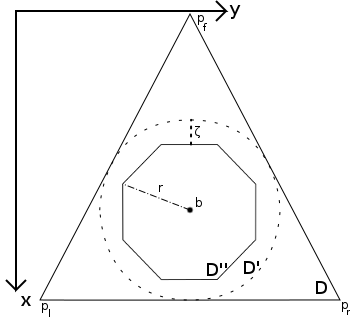
\includegraphics[width=4in]{ctr_base.png}
						\caption{Représentation des contraintes de non-basculement. $D$ correspond à la contrainte exacte.
							 $D'$ correspond à la contrainte circulaire inscrite dans $D$, rendant celle-ci invariante par rotation atour de $b$.
							 $D''$ correspond à la linéarisation de la contrainte $D'$ par un octogone, en ajoutant une marge de sécurité $\zeta$.}
						\label{fig.ctr_base2}
					}
				
				
					La contrainte principale à la stabilité de la commande est celle empêchant le robot de basculer \rfi{fig.ctr_base2}.
					Nous rappelons l'expression des contraintes de non-basculement \rf{eq.ctr_cop_1}\rf{eq.ctr_cop_2}\rf{eq.ctr_cop_3}.
					$\forall k \in (1, n)$ :
					\eqa{
						d^{xy}_k \times (p_r^{xy}-p_f^{xy}) &> 0 \\
						d^{xy}_k \times (p_l^{xy}-p_r^{xy}) &> 0 \\
						d^{xy}_k \times (p_f^{xy}-p_l^{xy}) &> 0
					}
					
					Ces contraintes ne sont pas invariantes par rotation de la base mobile.
					On réduit donc celles-ci à un cercle d'origine $B^{xy}$ que l'on linéarise par la suite par un octogone régulier de rayon $r'$, orienté selon la direction $\vec{x}$ \rfi{fig.ctr_base2}:
					\eqa{
						r' &= \min\prt{d_f, d_r, d_l} - \zeta  \\
						\zeta &>0
					}
					où $\zeta$ est une marge de sécurité. La formulation QP ne permet pas l'utilisation de contraintes d'inégalités strictes, la marge de sécurité $\zeta$ permet de s'en affranchir.
					
					Les contraintes linéarisées s'expriment donc directement de la façon suivante :
					\eq{
						v^-_1 \leq V_1X \leq v^+_1
					}
					avec
					\eqa{
					\nonumber
						V_1 &= \mat{
							U_{dc} & 0 & U_{db}-U_b & 0 \\
							0 & U_{dc} & 0 & U_{db}-U_b \\
							U_{dc} & U_{dc}  & U_{db}-U_b & U_{db}-U_b \\
							U_{dc} & -U_{dc}  & U_{db}-U_b & -U_{db}+U_b 
						}\\
					\nonumber
						v^-_1 &= \mat{
							-3\tilde{r}-S_{dc}\hat{c}^x-(S_{db}-U_b)\hat{b}^x \\
							-3\tilde{r}-S_{dc}\hat{c}^y-(S_{db}-U_b)\hat{b}^y \\
							-4\tilde{r}-S_{dc}(\hat{c}^x+\hat{c}^y)-(S_{db}-U_b)(\hat{b}^x+\hat{b}^y) \\
							-4\tilde{r}-S_{dc}(\hat{c}^x-\hat{c}^y)-(S_{db}-U_b)(\hat{b}^x-\hat{b}^y) 
						}\\
						v^+_1 &= \mat{
							3\tilde{r}-S_{dc}\hat{c}^x-(S_{db}-U_b)\hat{b}^x \\
							3\tilde{r}-S_{dc}\hat{c}^y-(S_{db}-U_b)\hat{b}^y \\
							4\tilde{r}-S_{dc}(\hat{c}^x+\hat{c}^y)-(S_{db}-U_b)(\hat{b}^x+\hat{b}^y) \\
							4\tilde{r}-S_{dc}(\hat{c}^x-\hat{c}^y)-(S_{db}-U_b)(\hat{b}^x-\hat{b}^y) 
						}
					}
					et $\tilde{r} = \dfrac{r'}{\sqrt{10}}$.
					
				
				\subsubsubsection{Vitesses et accélérations maximales de la base mobile}
				\label{section.ctr_base_3_roues}
				
				Les moteurs des roues de la base mobile sont limités en vitesse et accélération. Il faut donc prendre en compte cet élément afin de ne pas générer de commandes infaisables par le robot.
				Il n'y a pas de relation linéaire entre les limites cinématiques des moteurs des roues et celles de la base mobile.
				Nous allons donc définir des contraintes concernant la base mobile, conservatives vis à vis de celles des moteurs.
				
				Soit $\dot{b}_{m}$ et $\ddot{b}_{m}$ des limites en vitesse et accélération de la base mobile, nous pouvons exprimer les contraintes de la façon suivante.  
				$\forall k \in (1, n)$ :
				\eqa{
					\norm{\vec{\dot{b}}_k} &\leq \dot{b}_{m} \\
					\norm{\vec{\ddot{b}}_k} &\leq \ddot{b}_{m}
				}
				
				Ces contraintes étant non-linéaires, nous avons choisi de les approximer simplement par un carré, car, contrairement aux contraintes sur le CoP, celles-ci ne sont pas critiques concernant la stabilité du robot.
				Ainsi, même si les contraintes linéaires résultantes sont significativement non-conservatives par rotation du robot, cela n'impacte que de façon mineure le comportement de la commande.
				Cette solution est donc préférable, du point de vue du temps de calcul de la commande, au choix d'un polygone d'ordre plus élevé.
				
				
				Les contraintes linéarisées s'expriment donc de la façon suivante :
					\eq{
						v^-_2 \leq V_2X \leq v^+_2
					}
					avec :
					\eqa{
						V_2 &= \mat{
							0 & 0 & U_{\dot{b}} & 0 \\
							0 & 0 & 0 & U_{\dot{b}} \\
							0 & 0 & U_{\dot{b}} & 0 \\
							0 & 0 & 0 & U_{\dot{b}}
						},~~
						v^-_2 = \mat{
							-\tilde{\dot{b}}_m - S_{\dot{b}}\hat{b}^x \\
							-\tilde{\dot{b}}_m - S_{\dot{b}}\hat{b}^y \\
							-\tilde{\ddot{b}}_m - S_{\ddot{b}}\hat{b}^x \\
							-\tilde{\ddot{b}}_m - S_{\ddot{b}}\hat{b}^y \\
						},~~
						v^+_2 = \mat{
							\tilde{\dot{b}}_m - S_{\dot{b}}\hat{b}^x \\
							\tilde{\dot{b}}_m - S_{\dot{b}}\hat{b}^y \\
							\tilde{\ddot{b}}_m - S_{\ddot{b}}\hat{b}^x \\
							\tilde{\ddot{b}}_m - S_{\ddot{b}}\hat{b}^y \\
						}
					}
					et :
					\eqa{
						\tilde{\dot{b}}_m = \frac{\sqrt{2}}{2}\dot{b}_m \\
						\tilde{\ddot{b}}_m = \frac{\sqrt{2}}{2}\ddot{b}_m
					}
	
				
				\subsubsubsection{Limites articulaires du corps du robot}
				\label{section.ctr_body_3_roues}
			
					\fig{
						\centering
						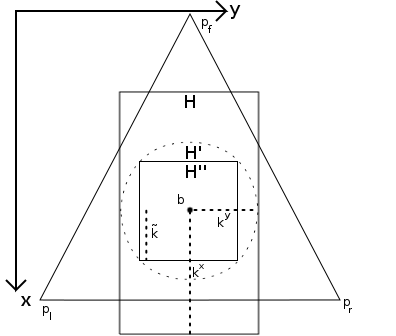
\includegraphics[width=4in]{ctr_body.png}
						\caption{Représentation des contraintes cinématiques du corps du robot. $H$ correspond à la contrainte exacte.
							 $H'$ correspond à la contrainte circulaire inscrite dans $H$, rendant celle-ci invariante par rotation autour de $b$.
							 $H''$ correspond à la linéarisation de la contrainte $H'$ par un carré.}
						\label{fig.ctr_body}
					}
					
					L'agencement des corps et articulations du robot implique que la distance entre son CoM $C^{xy}$ et celui de la base mobile $B^{xy}$ est limitée.
					Sur la plate-forme expérimentale, si l'on considère les approximations réalisées dans le chapitre \rf{chapitre.modele} ($c^z$ constant et on ignore les mouvements des bras),
					cette zone de déplacement correspond exactement à un rectangle centré autour de $B^{xy}$, de dimension $(2k^x, 2k^y)$ \rfi{fig.ctr_body}.
					
					Cette contrainte n'est pas invariante par rotation.
					Nous choisissons donc de réduire cette contrainte à un cercle centré autour de la base mobile $B^{xy}$, de rayon $\min\prt{k^x, k^y}$.
					Enfin, on linéarise ce cercle en un carré de dimension $2\tilde{k}$ \rfi{fig.ctr_body}, avec :
					\eq{
						\tilde{k} = \frac{\sqrt{2}}{2}\min\prt{k^x, k^y}
					}
					
					Nous ne choisissons pas ici un polygone d'ordre supérieur à $2$ car les limites articulaires du corps du robot sont dans la majorité des cas négligeables devant celles concernant le CoP.
					Ainsi, dans une situation normale, le robot ne se retrouve généralement pas en contrainte sur ses limites articulaires, ce qui rend un polygone d'ordre $2$ suffisant pour représenter les contraintes associées.
					
					Les contraintes linéarisées s'expriment donc de la façon suivante :
					\eq{
						v^-_3 \leq V_3X \leq v^+_3
					}
					avec
					\eqa{
						V_3 &= \mat{
							U_c & 0 & -U_b & 0 \\
							0 & U_c & 0 & -U_b
						},~~
						v^-_3 = \mat{
							-\tilde{k} - S_c\hat{c}^x + S_b\hat{b}^x \\
							-\tilde{k} - S_c\hat{c}^y + S_b\hat{b}^y
						},~~
						v^+_3 = \mat{
							\tilde{k} - S_c\hat{c}^x + S_b\hat{b}^x \\
							\tilde{k} - S_c\hat{c}^y + S_b\hat{b}^y
						}
					}
					
					

			\subsubsection{Problème quadratique résultant}
				\label{section.qp_3roues}
				
				La loi de commande optimale présentée possède plusieurs objectifs. Il existe classiquement deux manières de résoudre une problème multi-objectifs :
				\liste{
					\item Considérer une hiérarchie d'objectifs. A chaque niveau hiérarchique, un seul objectif est optimisé, ceux qui sont prioritaires sont considérés comme des contraintes, et les autres ne sont pas optimisés à ce niveau de hierarchie.
					\item Considérer une somme pondérée d'objectifs. Plus les pondérations associées sont relativement grandes les unes par rapport aux autres, plus les objectifs associés sont prioritaires.
				}
				
				Nous avons fait le choix de résoudre le problème par une somme pondérée d'objectifs. 
				Ce choix est motivé d'une part par le fait que les solveurs de QP que nous avions de disponibles ne permettent pas de résoudre un problème hiérarchique.
				D'autre part, en utilisant le principe d'une somme pondérée d'objectifs, nous pouvons tendre vers la première solution en augmentant l'écart relatif entre les pondérations de plusieurs ordres de grandeurs.
				Réaliser l'inverse n'est pas possible.
				
				Soit $\alpha_i$ la pondération associée à l'objectif $i$, nous pouvons écrire le problème quadratique résultant de la façon suivante :
				\eq{
					\lst{
						\min\limits_X \prt{\tr{X}\somme{i=1}{5}{\alpha_iQ_i}X+\somme{i=1}{5}{\alpha_i\tr{\rho}_i}X} \\
						\mat{v_1^- \\ v_2^- \\ v_3^-} \leq \mat{V_1 \\ V_2 \\ V_3} X \leq \mat{v_1^+ \\ v_2^+ \\ v_3^+}
					}
				}
				
				

		\subsection{Lorsque le robot bascule sur deux roues}
			\label{section.mpc_deux_roues}
			\subsubsection{Formulation des objectifs}
			
				Lorsque le robot bascule sur deux roues, nous pouvons définir trois objectifs de commande :
				\liste{
					\item Contrôler l'angle de basculement à $0$, afin de ramener le robot sur trois roues.
					\item Minimiser la vitesse angulaire de basculement. Cet objectif a pour but de limiter l'impact occasionné lorsque l'angle de basculement atteint $0$.
					      Si la vitesse angulaire est nulle au moment où la roue touche le sol, il n'y a pas d'impact.
					\item Assurer la stabilité numérique de la commande optimale. Cela peut être réalisé en minimisant le carré des variables de commande $X'$.
				}
				
				Dans la suite, nous noterons $O'_i$ l'objectif $i$. Il correspond à la norme élevée au carré d'une fonction des variables de commande. Il s'écrit de la façon suivante :
				\eq{
					O'_i = \frac{1}{2}\norm{f'_i(X)}^2
				}
				puis, en utilisant la notation QP :
				\eq{
					O'_i = \frac{1}{2}\tr{X}Q'_iX + \tr{\rho'}_iX + \epsilon'_i
				}
				avec $Q'_i$ une matrice symétrique définie positive (dite Hessienne), $\rho'_i$ un vecteur et $\epsilon_i$ un scalaire constant.
				Nous ne détaillerons pas l'expression des $\epsilon'_i$ car ce terme n'a pas d'impact pas dans la minimisation des l'objectifs $O'_i$.
				
				On rapelle le vecteur de commande dans le cas où le robot bascule sur deux roues :
				\eq{
					X' = \tr{\mat{\dddot{C}^n & \dddot{B}^n}}
				}
				
				\subsubsubsection{Minimisation de l'angle de basculement}
				
					L'objectif principal de la commande est d'assurer le retour sur trois roues au sol du robot en amenant l'angle de basculement à $0$.
					Nous pouvons donc écrire l'objectif $O'_1$ correspondant en utilisant l'équation \rf{eq.dyn_tilt_pred} :
					\eq{
						O'_1 = \frac{1}{2}\norm{\Psi}^2 = \frac{1}{2}\tr{X'}Q'_1X'+\tr{\rho'}_1X+\epsilon'_1
					}
					avec :
					\eqa{
					\nonumber
						Q'_1 &= \mat{
							\tr{U}_{\psi c}\tilde{U}^{-t}_{\psi}\tilde{U}^{-1}_{\psi}U_{\psi c} & \tr{U}_{\psi c}\tilde{U}^{-t}_{\psi}\tilde{U}^{-1}_{\psi}U_{\psi b} \\
							\tr{U}_{\psi b}\tilde{U}^{-t}_{\psi}\tilde{U}^{-1}_{\psi}U_{\psi c} & \tr{U}_{\psi b}\tilde{U}^{-t}_{\psi}\tilde{U}^{-1}_{\psi}U_{\psi b}	
						}\\
						\rho'_1 &= \mat{
							\tr{U}_{\psi c}\tilde{U}^{-t}_{\psi}(S_{\psi b}\hat{b}^n + S_{\psi c}\hat{c}^n + S_{\psi g^x}g^x + S_{\psi g^y} g^y + S_{\psi \psi} \hat{\psi}) \\
							\tr{U}_{\psi b}\tilde{U}^{-t}_{\psi}(S_{\psi b}\hat{b}^n + S_{\psi c}\hat{c}^n + S_{\psi g^x}g^x + S_{\psi g^y} g^y + S_{\psi \psi} \hat{\psi})
						}
					}
				
				\subsubsubsection{Minimisation de la vitesse angulaire}
				
					Afin de limiter l'impact du robot lorsqu'il touchera le sol, il est important de minimiser la vitesse angulaire de basculement.
					Pour exprimer l'objectif correspondant, il faut dans un premier temps écrire les relations entre la vitesse angulaire de basculement $\dot{\Psi}$ et les variables du problème $X'$.
					\eq{
						\dot{\Psi} = U_{\dot{\psi}}\dddot{\Psi} + S_{\dot{\psi}}\hat{\psi}
					}
					
					En utilisant l'équation \rf{eq.dyn_tilt_pred}, on peut donc écrire :
					\eq{
					\label{eq.dot_psi}
						\dot{\Psi} = U_{\dot{\psi}}\tilde{U}^{-1}_\psi \prt{U_{\psi b}\dddot{B}^n + U_{\psi c}\dddot{C}^n + S_{\psi b}\hat{b}^n 
						           + S_{\psi c}\hat{c}^n + S_{\psi g^x}g^x + S_{\psi g^y} g^y} + \prt{U_{\dot{\psi}} \tilde{U}^{-1}_\psi  S_{\psi \psi} + S_{\dot{\psi}}} \hat{\psi}
					}

					Nous pouvons donc écrire l'objectif $O'_2$ : 
					\eq{
						O'_2 = \frac{1}{2}\norm{\dot{\Psi}}^2 = \frac{1}{2}\tr{X'}Q'_2X'+\tr{\rho'}_2X+\epsilon'_2
					}
					avec :
					\eqa{
						\nonumber	
						Q'_2 &= \mat{
							\tr{U}_{\psi c}\tilde{U}^{-t}_\psi\tr{U_{\dot{\psi}}} U_{\dot{\psi}}\tilde{U}^{-1}_\psi U_{\psi c} & \tr{U}_{\psi c}\tilde{U}^{-t}_\psi\tr{U_{\dot{\psi}}} U_{\dot{\psi}}\tilde{U}^{-1}_\psi U_{\psi b} \\
							\tr{U}_{\psi b}\tilde{U}^{-t}_\psi\tr{U_{\dot{\psi}}} U_{\dot{\psi}}\tilde{U}^{-1}_\psi U_{\psi c} & \tr{U}_{\psi b}\tilde{U}^{-t}_\psi\tr{U_{\dot{\psi}}} U_{\dot{\psi}}\tilde{U}^{-1}_\psi U_{\psi b}  
						}\\
						\rho'_2 &= \mat{
							\tr{U}_{\psi c}\tilde{U}^{-t}_\psi\tr{U_{\dot{\psi}}} \prt{U_{\dot{\psi}}\tilde{U}^{-1}_\psi (S_{\psi b}\hat{b}^n + S_{\psi c}\hat{c}^n + S_{\psi g^x}g^x + S_{\psi g^y} g^y) + (U_{\dot{\psi}} \tilde{U}^{-1}_\psi  S_{\psi \psi} + S_{\dot{\psi}}) \hat{\psi}} \\
							\tr{U}_{\psi b}\tilde{U}^{-t}_\psi\tr{U_{\dot{\psi}}} \prt{U_{\dot{\psi}}\tilde{U}^{-1}_\psi (S_{\psi b}\hat{b}^n + S_{\psi c}\hat{c}^n + S_{\psi g^x}g^x + S_{\psi g^y} g^y) + (U_{\dot{\psi}} \tilde{U}^{-1}_\psi  S_{\psi \psi} + S_{\dot{\psi}}) \hat{\psi}} 
						}
					}
				
				\subsubsubsection{Stabilité numérique}
				
					Le dernier objectif concerne la stabilité numérique du problème d'optimisation.
					Afin de réaliser cela, une solution consiste à minimiser le jerk des commandes $\dddot{C}^{n}$ et $\dddot{B}^{n}$.
					
					Nous pouvons donc écrire le dernier objectif $O'_5$ :
					\eq{
						O'_3 = \frac{1}{2}\norm{X'}^2 = \frac{1}{2}\tr{X}Q'_3X + \tr{\rho'}_3X + \epsilon_3
					}
					avec : 
					\eq{
						Q'_3 = \id, ~~\rho'_3 = 0
					}

			\subsubsection{Formulation des contraintes}
			
				Lorsque le robot est en basculement sur deux roues, il est important de définir un certain nombre de contraintes :
				\liste{
					\item Respecter les contraintes de non-pénétrtation dans le sol, en assurant que l'angle de basculement $\Psi$ est toujours positif ou nul.
					\item Respecter les limites physiques de la base mobile en limitant les vitesses et accélérations maximales
					\item Respecter la cinématique du corps du robot, en limitant la distance entre son CoM $C^{xy}$ et celui de la base mobile $B^{xy}$.
				}
				
				Contrairement à la section \rf{ctr_intro_3_roues}, le robot ne peut pas tourner pendant le contrôle du basculement ($B^t$ et $C^t$ constant).
				Il n'est donc pas nécessaire de rendre les contraintes invariantes par rotation autour de la base $B$.
				
				Dans les sections suivantes, nous écrirons les contraintes linéarisées de la façon suivante :
				\eq{
					v'^-_i \leq V'_iX' \leq v'^+_i
				}
				
				\subsubsubsection{Contraintes de non-pénétration dans le sol}
				
					La présence du sol fait que l'angle de basculement $\Phi$ ne peut pas etre négatif.
					Cette contrainte est directement linéaire en les variables de commande et s'exprime ainsi :
					\eq{
						\Phi \ge 0
					}
					
					On peut donc écrire la contrainte de la façon standard :
					\eq{
						v'^-_1 \leq V'_1X' \leq v'^+_1
					}
					avec :
					\eqa{
					\nonumber
						V'_1 &= \mat{
							\tilde{U}^{-1}U_{\psi c} & \tilde{U}^{-1}U_{\psi b}
						} \\
					\nonumber
						v'^-_1 &= \mat{
							-\tilde{U}^{-1}\prt{S_{\psi b}\hat{b}^n + S_{\psi c}\hat{c}^n + S_{\psi g^x}g^x + S_{\psi g^y} g^y + S_{\psi \psi} \hat{\psi}}
						}\\
						v'^+_1 &= \mat{
							+\infty
						}
					}
				
				\subsubsubsection{Vitesses et accélérations maximales de la base mobile}
				
					De façon identique à la section \rf{section.ctr_base_3_roues}, les contraintes en vitesse et accélération de la base mobile s'écrivent de la façon suivante :	
					\eqa{
						\norm{\vec{\dot{b}}_k} &\leq \dot{b}_{m} \\
						\norm{\vec{\ddot{b}}_k} &\leq \ddot{b}_{m}
					}
					
					Le robot ne pouvant se déplacer qu'uniquement sur la droite représentée par le vecteur $\vec{n}_k$, les contraintes peuvent se réécrire de la façon suivante :
					\eqa{
						\dot{b}^n &\leq \dot{b}_{m} \\
						\ddot{b}^n &\leq \ddot{b}_{m} 
					}
					ce qui se réécrit de façon standard :
					\eq{
						v'^-_2 \leq V'_2X' \leq v'^+_2
					}
					avec :
					\eq{
						V'_2 = \mat{
							0 & U_{\dot{b}} \\
							0 & U_{\ddot{b}} \\
						},~~
						v'^-_2 = \mat{
							-\dot{b}_{m} - S_{\dot{b}}\hat{b}^n \\
							-\ddot{b}_{m} - S_{\ddot{b}}\hat{b}^n \\
						},~~
						v'^+_2 = \mat{
							\dot{b}_{m} - S_{\dot{b}}\hat{b}^n \\
							\ddot{b}_{m} - S_{\ddot{b}}\hat{b}^n \\
						}
					}					
				
				\subsubsubsection{Limites articulaires du corps du robot}
				
					\fig{
						\centering
						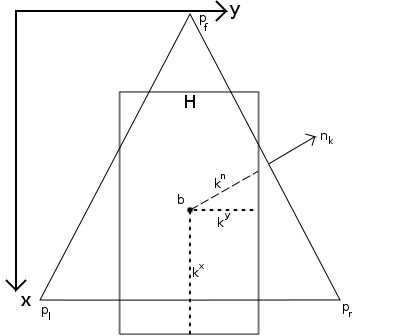
\includegraphics[width=4in]{ctr_body_tilt.png}
						\caption{Représentation des contraintes cinématiques du corps du robot lorsque celui-ci bascule. $H$ correspond à la contrainte exacte. 
						         $k^n$ correspond à la distance entre le point $b$ et le point d'intersection de l'axe $(b, \vec{n}_k)$ et l'enveloppe $H$}
						\label{fig.ctr_body_tilt}
					}
					
					De façon identique à la section \rf{section.ctr_body_3_roues}, on défini la contrainte entre le CoM du corps du robot $C$ et celui de la base mobile $B$ par un rectangle de dimensions $(k^x, k^y)$ centré en $b$.
					
					Soit $k^n$ la distance du segment reliant le centre de la base mobile $B$ et le point d'intersection entre la droite définie par le vecteur $\vec{n}_k$ et d'origine $B$ avec le rectangle de la contrainte. $k^n$ s'exprime de la façon suivante \rfi{fig.ctr_body_tilt} :
					\eq{
						k^n = \min\prt{
							\norm{k^x\cos(\theta_k)},
							\norm{k^y\sin(\theta_k)}
						}
					}
					
					La contrainte s'exprime de la façon suivante :
					\eq{
						-k^n \leq C^n-B^n \leq k^n
					}
					ce qui se réécrit de façon standard :
					\eq{
						v'^-_3 \leq V'_3X' \leq v'^+_3
					}
					avec :
					\eqa{
						V'_3 = \mat{
							U_c & -U_b
						},~~
						v'^-_3 = \mat{
							-k^n - S_c\hat{c}^n + S_b\hat{b}^n
						},~~
						v'^+_3 = \mat{
							k^n - S_c\hat{c}^n + S_b\hat{b}^n
						}
					}

			\subsubsection{Problème quadratique résultant}
		
				De la même manière qu'en section \rf{section.qp_3roues}, nous pouvons écrire le problème quadratique résultant de la façon suivante :
				\eq{
					\lst{
						\min\limits_{X'} \prt{\tr{X'}\somme{i=1}{3}{\alpha'_iQ'_i}X'+\somme{i=1}{3}{\alpha'_i\tr{\rho'}_i}X'} \\
						\mat{v'^-_1 \\ v'^-_2 \\ v'^-_3} \leq \mat{V'_1 \\ V'_2 \\ V'_3} X \leq \mat{v'^+_1 \\ v'^+_2 \\ v'^+_3}
					}
				}
				avec $\alpha'_i$ la pondération associée à l'objectif $O'_i$.

		\subsection{Gestion de la transition entre les deux états}
		\label{section.mpc_transition}
		
			Le contrôleur décrit en section \rf{section.mpc_deux_roues} ne prend pas en compte la force de réaction qui se rajoute au moment où l'angle de basculement atteint $0$.
			Cela amène ce contrôleur à générer une très grande accélération afin de maintenir l'angle à $0$. 
			Bien que celle-ci puisse être réalisable, ce comportement n'est pas souhaitable et nous préférons ``laisser tomber'' le robot sur le sol lorsque celui-ci va le percuter, afin d'éviter un déplacement exagéré de la base mobile.
			
			Il faut donc adjoindre aux deux précédents contrôleurs un troisième permettant de gérer cet état. Nous choisissons d'utiliser le jeu de variable $X$.
			Les objectifs choisis sont :
			\liste{
				\item $O_3$ et $O_4$. Contrôler le CoP au milieu de la base en utilisant le modèle de robot sur trois roues permet d'assurer au robot de ne pas accroitre son angle de basculement.
				      Cet objectif permet de contrôler le moment angulaire du robot autour de son axe de rotation afin qu'il soit toujours dirigé vers la bonne direction, lorsque celui-ci est proche du sol.
				\item $O_5$. Assurer la stabilité numérique de l'algorithme est toujours indispensable.
			}
			
			Les contraintes choisies sont :
			\liste{
				\item $(V_1, v^+_1, v^-_1)$. La contrainte sur le CoP permet d'assurer au robot que son moment angulaire va faire tomber celui-dernier sur ces trois roues, lorsque celui-ci est  proche du sol.
				\item $(V_2, v^+_2, v^-_2)$ et $(V_3, v^+_3, v^-_3)$. Afin de ne pas générer de mouvements infaisables, il faut contraindre le déplacement de la base mobile et du corps du robot.
			}
			
			Il faut cependant prendre en compte que le robot est toujours sous-actionné, car ayant une roue en l'air. 
			Il s'impose donc de rajouter une contrainte concernant le déplacement de la base mobile, qui doit se faire uniquement selon l'axe $\vec{n}_k$.
			Cette contrainte s'exprime de la façon suivante :
			\eq{
				\cos(\theta_k)\dot{B}^y = \sin(\theta_k)\dot{B}^x
			}
			ce qui se réécrit de façon standard :
					\eq{
						v^-_4 \leq V_4X \leq v^+_4
					}
					avec :
					\eqa{
					\nonumber
						V_4 &= \mat{
							0 & 0 & \sin(\theta_k)U_{\dot{b}} & - \cos(\theta_k)U_{\dot{b}}
						}\\
						v^-_4 &= v^+_4 = \mat{
							\cos(\theta_k)S_{\dot{b}}\hat{b}^y - \sin(\theta_k)S_{\dot{b}}\hat{b}^x
						}
					}

			Le problème quadratique résultant s'écrit donc :
			\eq{
				\lst{
					\min\limits_{X} \prt{\tr{X}\somme{i=3}{5}{\alpha_iQ_i}X'+\somme{i=3}{5}{\alpha_i\tr{\rho}_i}X} \\
					\mat{v^-_1 \\ v^-_2 \\ v^-_3 \\ v^-_4} \leq \mat{V_1 \\ V_2 \\ V_3 \\ V_4} X \leq \mat{v^+_1 \\ v^+_2 \\ v^+_3 \\ v^+_4}
				}
			}
			

	\section{Gestion des deux modèles dynamiques exclusifs}
		\label{section.superviseur}
		\subsection{Choix d'un superviseur et conséquences}
		
			L'objectif est maintenant de définir un moyen permettant de choisir quel contrôleur parmi les trois proposés en sections \rf{section.mpc_trois_roues}\rf{section.mpc_deux_roues}\rf{section.mpc_transition} doit être activé afin de commander le robot.
			Nous avons fait le choix d'un superviseur basé sur une machine a états et d'une heuristique de transition entre ces états.
		
			Les avantages de ce type de superviseur sont qu'il est facile à implémenter ainsi qu'à en faire évoluer les paramètres associés aux heuristiques de transition.
			De plus, ce type de superviseur permet de gérer de façon simple les transitions de modes dynamiques ainsi que les impacts.
			
			Les inconvénient sont le fait que l'utilisation d'heuristiques rend le comportement du robot non-optimal à une situation donné.
			De plus, si celles-ci sont mal choisies, son comportement peut être contraire aux objectifs de commande et impacter négativement son équilibre. 
			Nous verrons notament les conséquences de l'utilisation d'heuristiques de transitions au chapitre \rf{chapitre.resultats}
			
			Dans la suite, il est important de prendre en compte au fait que certaines heuristiques ont été faites pour prendre en compte les perturbations les plus communes qu'un humain peut appliquer à la plate-forme expérimentale.
			
		\subsection{Fonctionnement du superviseur}

			\fig{
				\centering
				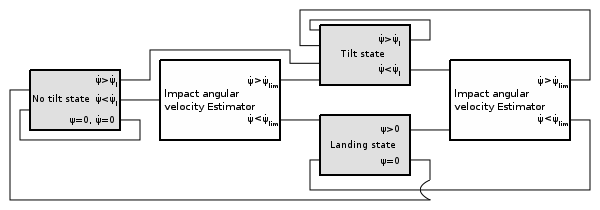
\includegraphics[width=6.5in]{supervisor.png}
				\caption{Schéma de fonctionnement du superviseur. 
					Les boites ``No tilt state'', ``Tilt state'' et ``Landing state'' correspondent aux états du superviseur.
					Les boites ``impact angular velocity estimator'' correspondent à l'estimateur de vitesse d'impact, permettant de gérer la transition entre les états.}
				\label{fig.supervisor}
			}
			
			\subsubsection{Les états du superviseur}
				
				
				La machine à états du superviseur est composé de trois états \rfi{fig.supervisor} :
				\liste{
					\item L'état \textit{No tilt} indique que le robot possède les trois roues sur le sol. Le contrôleur développé en section \rf{section.mpc_trois_roues} est donc activé.
					\item L'état \textit{Tilt} indique que le robot est en basculement sur deux roues. Le contrôleur développé en section \rf{section.mpc_deux_roues} est donc activé.
					\item l'état \textit{Landing} indique que le robot est en basculement sur deux roues, mais proche du sol et sur le point de le toucher. Le contrôleur développé en section \rf{section.mpc_transition} est donc activé.
				}
				
				Afin de définir les transitions entre les états, trois mesures sont utilisées : l'angle de basculement, la vitesse angulaire, et l'estimation de la vitesse angulaire d'impact.
			
			\subsubsection{Les transitions depuis l'état \textit{No tilt}}
			
				Lorsque le superviseur est dans l'état \textit{No tilt}, les transitions sont les suivantes \rfi{fig.supervisor} :
				\liste{
					\item Si la vitesse angulaire mesurée est supérieure à une limite donnée $\psi_l$, alors le superviseur passe à l'état \textit{Tilt}. 
					On ne peut pas prévoir la durée ni l'intensité de la perturbation dans le futur.
					Ainsi, si on mesure une forte vitesse angulaire, on suppose que l'humain qui pousse le robot ne va pas arrêter son geste rapidement, au moins pour des raisons d'inertie.
					
					\item Si la vitesse angulaire est inférieure à $\psi_l$, mais non-nulle, on utilise un estimateur de vitesse angulaire d'impact (qui sera décrit en section \rf{section.impact_estimator}).
					Si celui-ci indique que, sans compensation active par le contrôleur \rf{section.mpc_deux_roues}, le robot va tomber ou avoir une trop grande vitesse angulaire estimée au moment de l'impact, alors le superviseur passe à l'état \textit{Tilt}.
					Cet estimateur permet de déterminer si le robot va tomber, en considérant un arrêt de la force de perturbation et une absence de compensation par le contrôleur \rf{section.mpc_deux_roues}.
					Si non, cet estimateur indique la vitesse angulaire d'impact.
					
					\item Dans le cas où l'estimateur indique que la vitesse angulaire d'impact estimée est suffisamment faible, alors le superviseur passe à l'état \textit{Landing}.
					Cela signifie que le robot va compenser passivement la perturbation et ne pas générer un impact trop élevé. 
					Dans ce cas, le mieux est de stopper le suivi de trajectoire, ainsi que de limiter le déplacement du robot dans l'axe de basculement, ce qui correspond bien au contrôleur de l'état \textit{Landing}.
					
					\item Dans tout les autres cas, le superviseur reste dans l'état \textit{No tilt}, car il n'est pas en train de basculer.
				}
				
			\subsubsection{Les transitions depuis l'état \textit{Tilt}}
			
				Lorsque le superviseur est dans l'état \textit{Tilt}, les transitions sont les suivantes  \rfi{fig.supervisor} :
				\liste{
					\item Si la vitesse angulaire mesurée est supérieure à $\psi_l$, alors le superviseur reste dans l'état \textit{Tilt}. 
					      Cela signifie que la perturbation n'a toujours pas été contrôlée.
					\item Dans le cas contraire, on utilise l'estimateur afin de déterminer la vitesse angulaire d'impact. 
					      Si celle-ci est trop forte, alors le superviseur reste dans l'état \textit{Tilt}.
					\item Dans le cas contraire, le superviseur passe à l'état \textit{Landing}.
					      Cela signifie que la perturbation a été suffisamment compensée pour à présent laisser tomber le robot sur le sol et finir de compenser passivement la perturbation.
				}
			
			\subsubsection{Les transitions depuis l'état \textit{Landing}}
			
				Lorsque le superviseur est dans l'état \textit{Landing}, les transitions sont les suivantes  \rfi{fig.supervisor} :
				\liste{
					\item Lorsque la vitesse angulaire et l'angle de basculement atteind $0$, après une légère période de temporisation afin d'éviter tout rebond éventuel, le superviseur passe à l'état \textit{No tilt}.
					\item Dans le cas contraire, on utilise l'estimateur afin de déterminer la vitesse angulaire d'impact. Si celle-ci est trop grande, alors le superviseur passe à l'état \textit{Tilt}.
					\item Dans le cas contraire, alors la phase atterrissage n'est pas terminée et le superviseur reste dans l'état \textit{Landing}.
				}
			

		\subsection{Fonctionnement de l'estimateur d'impact}
		\label{section.impact_estimator}

			Le premier objectif de l'estimateur d'impact est de déterminer si le robot va pouvoir compenser passivement la perturbation, ou bien tomber.
			Le second objectif est, dans le cas où le robot va pouvoir compenser passivement la perturbation, estimer la vitesse angulaire au moment de l'impact.
			
			L'estimateur utilise l'observation courante de l'angle de basculement ainsi que la mesure de la vitesse angulaire.
			On suppose dans un premier temps que le robot a une accélération angulaire constante dépendant uniquement de la gravité et de l'angle actuel de basculement :
			\eq{
			\label{eq.ddot_psi_estimateur}
				\ddot{\psi} = -\frac{g^z}{h_b}\cos\prt{\psi_0+$atan$\prt{\dfrac{h_b}{d_k}}}
			}
			
			A l'aide de l'équation \rf{eq.ddot_psi_estimateur}, on peut écrire l'évolution de l'angle de basculement au cours du temps :
			\eq{
				\psi = -\frac{g^z\cos\prt{\psi_0+$atan$\prt{\dfrac{h_b}{d_k}}}}{2h_b}t^2+\dot{\psi}_0t+\psi_0
			}
			
			En résolvant l'équation quadratique associée, pour $\psi=0$, on peut déterminer si le robot va impacter le sol, et si oui, estimer quel va être la vitesse angulaire d'impact.
			Soit $\Delta$ tel que :
			\eq{
				\Delta = \dot{\psi}_0^2+\dfrac{2g^z\psi_0\cos\prt{\psi_0+$atan$\prt{\dfrac{h_b}{d_k}}}}{h_b}
			}
			
			Si $\Delta<0$, le robot va tomber et il n'y aura pas d'impact de la roue en l'air sur le sol.
			Dans le cas contraire, le temps d'impact $t_i$ est calculé de la manière suivante :
			\eq{
				t_i = \dfrac{h_b(\dot{\psi}_0\pm \sqrt{\Delta})}{g^z\cos\prt{\psi_0+$atan$\prt{\dfrac{h_b}{d_k}}}}
			}
			et la vitesse d'impact estimée $\dot{\psi}_i$ est :
			\eq{
				\dot{\psi}_i = -\sqrt{\Delta}
			}

	\section{Vers une modélisation unifiée des deux dynamiques}
	\label{section.modelisation_unifiee}
	
		Dans cette section, nous présentons une méthode de résolution du problème d'unification des deux modèles dynamiques \rf{eq.dyn_cop_pred}\rf{eq.dyn_tilt_pred}.
		nous n'avons pas eu le temps d'implémenter cette méthode sur la plate-forme expérimentale, nous allons donc apporter uniquement un début d'approche théorique.
		
		Afin d'unifier les deux modèles dynamiques en un seul contrôleur, tout en restant dans le formalisme de la programmation quadratique linéaire, 
		une solution est de résoudre \textit{a priori} le problème d'optimisation sur l'ensemble de l'horizon de prédiction.
		Nous proposons l'heuristique suivante :
		\liste{
			\item 	Dans le cas où le robot possède initialement les trois roues en contact avec le sol, on considère que celui-ci le restera durant tout l'horizon de prédiction. 
				La loi de commande utilisée est directement celle présentée en section \rf{section.mpc_trois_roues}.
			\item 	Dans le cas où le robot est initialement en basculement sur deux roues (suite à une forte perturbation par exemple), on considère que celui-ci le restera sur l'intervalle $[0, m]$ de l'horizon de prédiction, où $m\leq n$.
				La loi de commande utilisée sur cet intervalle est de la forme de celle présentée en section \rf{section.mpc_deux_roues}
				Sur l'intervalle  $[m+1, n]$, si celui-ci existe ($m<n$), on considère que le robot est revenue sur ses trois roues.
				La loi de commande utilisée sur cet intervalle est de la forme de celle présentée en section \rf{section.mpc_trois_roues}.	
		}
		
		Cette heuristique implique notament le fait que lorsque le robot est en basculement sur deux roues, celui-ci va soit le rester durant tout l'horizon, soit retomber sans rebondir à l'instant $m$. 
		Cela est théoriquement pris en compte par les contraintes sur le CoP sur l'intervalle $[m+1, n]$, assurant au robot de ne pas rebondir.
		Il faut pour cela intégrer dans la formulation du CoP sur les instants $[m+1, n]$ l'influence de la vitesse et de l'accélération angulaire d'impact sur la formulation du CoP.
		
		De plus, une prédiction de la valeur de $m$ doit être faite. 
		Il faut donc, en s'inspirant de l'estimateur d'impact par exemple \rf{section.impact_estimator}, prédire cet instant $m$ et s'assurer qu'il converge vers la véritable valeur au fur et à mesure que $m$ tend vers $0$.
		
		Enfin, un travail de réécriture de la dynamique future doit être faite, de façon analogue à ce qui a été fait en section \rf{section.modele_futur}, afin de prendre en compte les deux modèles, ainsi que de leur transition entre les instants $m$ et $m+1$.
		
		
	\section{Conclusion}
	
		Dans ce chapitre, nous avons présenté une loi de commande composite permettant de contrôler l'équilibre et les mouvements d'un robot humanoïde à roues omnidirectionnelles.
		Celle-ci se base sur trois sous-lois de commandes optimales utilisant le formalisme de la programmation quadratique et supervisées par une machine a état.
		Ces trois lois permettent de contrôler le robot dans des situations différentes :
		\liste{
			\item Lorsque le robot est en contact sur le sol avec ces trois roues.
			\item Lorsque le robot bascule sur deux roues.
			\item Lorsque le robot va impacter le sol.
		}
		En estimant l'existence et la vitesse angulaire future d'impact du robot avec le sol, ainsi qu'en mesurant l'angle de basculement courant et sa vitesse angulaire, le superviseur est capable de choisir quelle sous-loi de commande activer à chaque instant.
		
		Enfin, l'ébauche d'une approche unifiée de cette loi de commande a été présentée afin de se passer de l'utilisation d'un superviseur, ainsi que d'améliorer la gestion de la transition entre les deux modes dynamiques (trois ou deux roues en contact avec le sol).
		
		
		
\chapter{Mesures et observateurs}
	\section{Introduction}
	
		L'objectif de ce chapitre est de présenter les différentes mesures et observateurs qui sont nécessaires à la réalisation de la commande présentée en chapitre \rf{chapitre.commande}.
		Nous présenterons dans un premier temps les différentes valeurs à observer, puis la liste des capteurs diponibles sur la plate-forme expérimentale.
		Ensuite de quoi, nous détaillerons les méthodes de mesures ainsi que les observateurs permettant de réaliser cela. 
		Enfin, nous discuterons des conséquences de chaque méthode sur la stabilité et le comportement final du robot.
		
		Les observateurs présentés dans ce chapitre ont été implémentés directement sur la plate-forme expérimentale. 
		Les performances obtenues sur le robot n'étant pas limités par ceux-ci, ils ont volontairement été réalisés de façon simple.
		Le contenu de ce chapitre sera donc court, et ne traitera pas en détail de problématiques comme les bruits capteurs ou l'impact des incertitudes du modèle du robot sur les observations.
	
	\section{Valeurs à observer et capteurs disponibles}
	
		La loi de commande présentée en chapitre \rf{chapitre.commande} nécessite plusieurs variables d'entrées :
		\liste{
			\item L'état complet du CoM du corps du robot $\hat{c}$.
			\item L'état complet du CoM de la base mobile $\hat{b}$.
			\item L'angle de basculement et la vitesse angulaire, nécessaires au fonctionnement du superviseur \rf{section.superviseur}.
			\item L'orientation du sol, nécessaire au calcul du vecteur gravité $g$.
		}
		
		Afin de mesurer ces valeurs, la plate-forme expérimentale dispose de plusieurs capteurs :
		\liste{
			\item	Associé à chaque moteur, des capteurs magnéto-résistifs permettent de mesurer son angle ou sa vitesse angulaire.
				Ces capteurs servent à mesurer la vitesse angulaire des roues de la base mobile.
				Sur chacune des articulation du robot, ces capteurs servent à mesurer l'angle de l'articulation.
			\item	Une centrale inertielle, disposée au centre de la base mobile, permet de mesurer l'accélération linéaire ainsi que la vitesse de rotation de la base mobile.
		}
		
		Nous pouvons constater dans un premier temps qu'aucune des variables d'entrée de la loi de commande n'est directement mesurée par les capteurs.
		Nous allons devoir réaliser des observateurs, afin d'estimer au mieux possibles ces valeurs.

	\section{Méthodes de mesure et conséquences}
		\subsection{Observation de l'état du CoM de la base mobile}
		
		\label{section.observateurbase}	
			\subsubsection{Vitesse du CoM de la base mobile}
			
				Les capteurs magnéto-résistifs associés aux moteurs des roues du robots nous permettent de mesurer la vitesse de rotation de celles-ci.
				En utilisant le modèle géométrique de la base mobile, nous pouvons en déduire directement une vitesse de déplacement de la base mobile.
				Cette déduction est valable uniquement si les roues ne glissent pas sur le sol.
				
				Soit $\beta_i$ la vitesse de la roue $i \in \{f, r, l\}$ et $W$ une matrice de transformation utilisant le modèle géométrique de la base mobile pour exprimer la vitesse de déplacement de la base mobile en fonction de celles des roues :
				\eq{
					\mat{\dot{b}^x \\ \dot{b}^y} = W\mat{\beta_f \\ \beta_r \\ \beta_l}
				}
				
				Les différences entre la vitesse réelle de la base mobile et celle observée proviennent directement des glissements entre les roues et le sol, dépendants de la nature du sol et de l'usure du revêtement des roues.
				
				Une méthode, qui n'a pas été implémentée, afin de mesurer ce glissement serait d'utiliser les accéléromètres de la centrale inertielle de la base mobile. 
			
			\subsubsection{Position du CoM de la base mobile}
			
				La position de la base mobile est directement obtenue par intégration des vitesses mesurées :
				\eq{
					\mat{b^x_\tau \\ b^y_\tau} = \mat{b^x_{0} \\ b^y_{0}} + \tau \mat{\dot{b}^x_0 \\ \dot{b}^y_0}
				}
				avec $\tau$ la période d'échantillonage de la mesure des $\beta_i$.
				
				Le défaut de cette approche est une dérive de la position du robot dans le temps. 
				Afin de compensser cette dérive lorsque le robot est immobile, principalement à cause du bruit capteur, un filtre en amplitude à été ajouté, ignorant les mesures de faible amplitude.
				
			\subsubsection{Accélération du CoM de la base mobile}
			\label{section.observation_acc_base}
				Concernant l'observation de l'accélération de la base mobile, le bruit de quantification apporté par une dérivation d'Euler de la vitesse mesurée ne nous permet pas d'obtenir une valeur utilisable.
				La solution qui a été choisie est d'utiliser l'équation d'état \rf{eq.dynamique_ordre_3} conjointement à la sortie de la loi de commande $X$ calculé au pas de temps précédent :
				\eq{
					\ddot{b}^x_\tau = \tau\dddot{B}(0) + \mat{0 & 0 & 1}\hat{b}_0
				}
				où $*(0)$ correspond à la première valeur du vecteur $*$.
				
				Si la commande $\dddot{B}(0)$ est bien réalisée par les moteurs, et en l'absence de perturbations, alors l'accélération observée $\ddot{b}^x_\tau$ correspond exactement à la valeur réelle.
				Les informations des erreurs générées par les perturbations vont cependant arriver avec un certain retard, dépendant des observations aux instants précédents de $b^x$ et $\dot{b}^x$.
				
				On peut noter que les accéléromètres présents dans la base mobile ne permettent pas de mesurer correctement $\ddot{b}$ car ceux-ci sont trop bruités.
				
		\subsection{Observation de l'état du CoM du corps du robot}
			\subsubsection{Position du CoM du corps du robot}
			
				Le corps du robot étant mécaniquement lié à la base mobile, on peut composer la position de son CoM en utilisant sa posture et la position du CoM de la base mobile $b$ :
				\eq{
					c = b + \delta_c
				}
				Où $\delta_c = c-b$, correspond aux informations apportées par la posture du robot.
				
				En utilisant le modèle géométrique du robot, ainsi que les capteurs de position articulaire, nous pouvons directement mesurer la valeur $\delta_c$.
				Cette mesure est valable tant que le modèle géométrique correspont au corps du robot. Ainsi, les déformations pouvant apparaître dans la structure du robot ne sont pas prises en compte.
		
			\subsubsection{Vitesse et accélération du CoM de la base mobile}
			
				Nous ne disposons d'aucune mesure de vitesse et d'accélération. 
				De plus, dériver directement la position du robot $c$ apporte beaucoup trop de bruit de quantification.
				Nous allons procéder de la même manière qu'en section \rf{section.observation_acc_base}, en utilisant l'équation d'état \rf{eq.dynamique_ordre_3} et la commande $X$ :
				\eqa{
					\dot{c}^x_\tau &= \frac{\tau^2}{2}\dddot{C}(0) + \mat{0 & 1 & \tau}\hat{c}_0 \\
					\ddot{c}^x_\tau &= \tau\dddot{C}(0) + \mat{0 & 0 & 1}\hat{c}_0
				}
				
			
		\subsection{Observation de l'angle de basculement et d'inclinaison du sol}
		\label{section.mesure_tilt_pente}
		
			Le capteur disponible permettant d'oserver l'angle de basculement et l'inclinaison du sol est la centrale inertielle disposée dans la base mobile.
			Le problème principal étant que ce capteur ne peut mesure que la somme des deux angles et vitesses angulaires.
			Sans utilisation d'\textit{a priori}, le système est donc non observable.
			
			Dans le chapitre \rf{chapitre.modele}, nous avons fait l'hypothèse d'une inclinaison du sol constante.
			Afin de rendre le système observable, nous allons donc définir les \textit{a priori} suivants :
			\liste{
				\item Lorsque la vitesse anglaire mesurée est nulle durant un temps minimum défini, on considère l'angle de basculement nul également. L'angle mesuré par la centrale inertielle correspond alors à l'inclinaison du sol.
				\item Lorsque la vitesse angulaire mesurée est non-nulle durant un temps minimum défini, on considère l'inclinaison du sol constante. L'angle et la vitesse angulaire mesurés correspondent donc au basculement du robot.
			}
			
			Deux cas limites émergent de ces \textit{a priori} :
			\liste{
				\item A cause du bruit capteur sur les gyromètres, si l'on amène le robot à basculer suffisamment lentement afin que la vitesse angulaire soit inférieure au bruit, alors il n'est pas possible de savoir que le robot est en train de basculer.
				      Cela peut être résolu par un capteur de force sur chaque roue, permettant de connaître exactement quelle roue est en l'air, et lesquelles sont au sol.
				      Dans notre cas, on suppose que cela n'arrive pas.
				\item Pendant le moment où le robot monte une pente, celle-ci est confondue avec un basculement, ce qui peut générer une commande non correcte du robot (accélération de la base mobile dans le sens descendant de la pente).
				      Cela est résolue par la temporisation minimum a partir duquel le robot change d'{a priori}, en considérant que le profil spatial d'inclinaison du sol est à variation nulle par morceaux 
				      (les changements d'inclinaison du sol sont spatialement instantanés, ce qui est le cas de la majorité des pentes que l'on peut croiser dans l'environement urbain).
				      
			}
			
			Mis à part ces deux cas limites, l'utilisation de ces \textit{a priori} permet d'observer simultanément l'angle de basculement et l'inclinaison du sol.
			Concernant la vitesse angulaire, celle-ci est directement extraite à partir des gyromètres, préalablement filtrés.
			Quant-à l'angle de basculement/d'inclinaison, celui-ci est calculé en utilisant un algorithme présenté dans l'article %\rf{}
			

			
\chapter{Résultats et expérimentations}

	\section{Schéma de contrôle en boucle fermée}
	\label{section.closedloop}

	- Présenter les asservissements bas niveau (feedback)
	
	- Parler de la cinématique inverse
	
	- feedback en position de mpc
	
	- Extrapolation pour compenser le retard capteur
	
	- Stabilisation en utilisant seulement une partie de sensor
	
	- Rejeter le jeu mécanique (threshold)
	
	\section{Expériences en l'absence de perturbation et sur sol horizontal}
		\subsection{Protocole expérimental}
		
			- Trajectoire non réalisable (test de faisabilité)
			
			- Variables : jeu de pondération / nombre de masses pendule / open et close-loop mpc
			
			- Trajectoire réalisable (test de suivi)
			
			- Influence des compensations retard capteur / command sensor / jeu mécanique 
		
		\subsection{Analyse des expériences}
		
			- Intérêt du choix des pondérations
			
			- Vers une adaptation automatique des pondérations
			
			- Intérêt d'une boucle fermée plus rapide que l'échantillonage du mpc
			
			- Utilisation de deux masses au lieu d'une
			
			- Influence de la compensation du retard dans le suivi de trajectoire
			
			- Nécessité de rejeter le jeu mécanique
			
			- Dû aux bruits, ne pas utiliser entièrement sensor
		
	\section{Expériences de compensation de perturbations}
		\subsection{Protocole expérimental}
		
			- Faire basculer le robot
			
			- Variable : Durée / puissance push / direction
			
		\subsection{Analyse des expériences}
		
			- Pas de recovery quand il n'y a pas besoin
			
			- Minimisation de la vitesse d'impact (le robot peut reculer)
		
			- Pousser trop fort emmènent aux limites physique du robot
			
			- Vers une utilisation des bras pour rééquilibrer
		
		
	\section{Expériences de compensation de l'inclinaison du sol}
		\subsection{Protocole expérimental}
		
			- Faire rouler le robot préalablement sur une pente
			
			- Faire monter / descendre une pente
			
			- Modifier la direction de déplacement
			
			- Modifier la nature du sol
			
			- Push sur pente
			
			- Pente variable
		
		\subsection{Analyse des expériences}
		
			- Vitesse limitée car roues qui décolle
			
			- Problème de détection push / pente
			
			- Compensation jusqu'à 5 degrés
			
			- Problèmes de glissement au delà
			
			- Cas limite de push pendant une montée de pente
		
\chapter{Synthèse}

	\section{Contributions}
	\section{Perspectives}
	\section{conclusion}

\addcontentsline{toc}{chapter}{Bibliographie}
\bibliography{bib}

\addcontentsline{toc}{chapter}{Annexes}
\appendix
\chapter{Optimisation du choix du modèle dynamique}
\chapter{Résolution d'un problème quadratique}

	
\end{document}